\documentclass[11pt,a4paper]{article}

\usepackage[margin=1.25in]{geometry}
\usepackage{amsmath,amssymb}
\usepackage{booktabs}
\usepackage{graphicx}
\usepackage{hyperref}
\usepackage{xcolor}
\usepackage{caption}
\usepackage{subcaption}
\usepackage{microtype}
\usepackage{parskip}
\usepackage{natbib}

\hypersetup{colorlinks=true, linkcolor=blue, citecolor=blue, urlcolor=blue}

\title{\textbf{Energy-Based Language Models at Scale: \\
Multi-Block Ablation and Curl--Gradient Structure}}
\author{Nima Dehmamy \\ IBM Research}
\date{April 2026}

\begin{document}
\maketitle

\begin{abstract}
We study energy-based transformer (EGPT) architectures at the 160M--400M parameter scale,
trained on the Nematron web-CC-HQ corpus with the dolomite-engine framework.
Each EGPT block performs an implicit gradient-descent step on a learned energy function,
parametrised by a dual-stream projection ($\mathrm{proj\_attn}$, $\mathrm{proj\_mlp}$) whose
symmetric part drives descent and anti-symmetric part drives conservative rotation.
We ablate five architectural choices---distinct vs.\ shared backbone, number of recurrence
steps, and learning rate---and evaluate on language modeling perplexity plus nine zero-shot
commonsense benchmarks, MMLU, and GSM8K.
The main finding is negative on compute efficiency: a 162M standard GPT baseline
consistently outperforms all 160M EGPT variants on perplexity, and a 400M EGPT model
requires 4.4$\times$ more FLOPs per token to approximately match the 162M GPT baseline
on perplexity and zero-shot accuracy.
EGPT appears significantly less compute-efficient than standard GPT at current scales.
We also analyze the Helmholtz decomposition of the projection matrices:
for all trained variants the curl-to-gradient ratio $\|A\|_F / \|S\|_F$ is close to 1,
confirming that the trained dynamics require a balanced mix of dissipation and rotation.
\end{abstract}

%% ============================================================
\section{Introduction}
%% ============================================================

Standard transformer residual blocks update the hidden state as
\[
  x_{t+1} = x_t + f(x_t),
\]
where $f$ is attention or FFN.  Energy-based variants instead perform
\[
  x_{t+1} = x_t - \mathrm{proj}(f(\mathrm{LN}(x_t))),
\]
which can be interpreted as a step of gradient descent on an implicit energy function
$E(x) \approx x^\top \mathrm{proj}(f(x))$.
Under the \emph{dual-unconstrained} parametrisation, the projection matrix
$W \in \mathbb{R}^{d \times d}$ is unconstrained, and via the Helmholtz decomposition
\[
  W = S + A, \quad S = \tfrac{1}{2}(W + W^\top), \quad A = \tfrac{1}{2}(W - W^\top),
\]
the symmetric part $S$ corresponds to pure gradient descent while the anti-symmetric part $A$
drives conservative (curl) dynamics, analogous to the dissipative ($R$) and conservative ($J$)
components in Port-Hamiltonian systems.

Prior work on a 410M hybrid model showed that the trained projection matrices converge to a
balanced mix ($\|S\|_F \approx \|A\|_F$) and that any deviation from this balance
severely degrades performance (prior alpha-sweep experiments, April 2026).
The present report scales these experiments to the fully-EGPT 160M--400M regime and ablates
the key design degrees of freedom.

%% ============================================================
\section{Model Architectures}
%% ============================================================

All models use the dolomite-engine \texttt{energy} model type with RoPE positional encoding,
RMSNorm, SwiGLU FFN, tied embeddings, and \texttt{dual\_unconstrained} projection.
Table~\ref{tab:variants} summarises the five variants.

\begin{table}[h]
\centering
\caption{Model variants in the 160M-scale multi-block ablation.
  ``Shared backbone'' ties the attention, FFN, and layer-norm weights across all 12 blocks
  (only $\mathrm{proj\_attn}$/$\mathrm{proj\_mlp}$ remain independent).}
\label{tab:variants}
\resizebox{\textwidth}{!}{%
\begin{tabular}{llccccc}
\toprule
\textbf{Variant} & \textbf{Description} & $d$ & \textbf{Blocks} & \textbf{Iters/block} & \textbf{Params} & \textbf{LR} \\
\midrule
V0 GPT    & Standard GPT (no energy proj)  & 768  & 12 distinct & 1 & $\sim$162M & 3e-4 \\
V1        & Distinct EGPT blocks            & 768  & 12 distinct & 1 & $\sim$143M & 3e-4 \\
V1 lr=2e-3 & V1 with higher LR             & 768  & 12 distinct & 1 & $\sim$143M & 2e-3 \\
V2        & Fewer distinct blocks           & 768  &  6 distinct & 2 & $\sim$110M & 3e-4 \\
V3        & Shared backbone                 & 1152 &  1 shared   & 12 & $\sim$163M & 3e-4 \\
V4        & Shared backbone, wide heads     & 1152 &  1 shared   & 12 & $\sim$349M$^\ddagger$ & 3e-4 \\
\bottomrule
\end{tabular}}
{\footnotesize $^\ddagger$ V4 without weight tying trains independent parameters per block; intended size was $\sim$174M.}
\end{table}

\paragraph{V0 GPT baseline.}
Standard decoder-only transformer.
Requires \texttt{num\_iterations: 0} in config to bypass the EGPT recurrence loop.

\paragraph{V1 / V2 EGPT (distinct blocks).}
Twelve (V1) or six (V2) independently-parametrised energy blocks.
Each block holds its own attention, FFN, layer-norm, and projection weights.
V2 applies each block twice (\texttt{layer\_iterations: [2]*6}).

\paragraph{V3 / V4 Shared backbone.}
A single attention+FFN backbone is shared across all 12 iterations, with only the
projection matrices $\{W^{(i)}_{\mathrm{attn}}, W^{(i)}_{\mathrm{mlp}}\}_{i=1}^{12}$
kept distinct.
V4 widens the attention heads to $\mathrm{head\_dim} = 288$ (4$\times$ the $d/n_h = 64$
standard) via expanded key/value projections.

\paragraph{400M scale (V1).}
A 24-layer, $d=1024$ version of V1 with 16 attention heads (\texttt{rope\_dim=64}),
intermediate size 3072, and LR=$7\times10^{-4}$ (muP scaling: $2\text{e-3} \times 768/1024$).
Trained for 30k steps (7.86B tokens), matching the token budget of V0 GPT.
\emph{Motivation:} WandB training curves showed the 400M EGPT loss closely tracking the
162M GPT loss curve, suggesting the two models have similar effective capacity despite the
large parameter count difference.
This run was designed to confirm whether benchmarks also match --- i.e., whether the
training loss alignment reflects genuine capability parity or a perplexity artefact.
Note: a compute-fair comparison requires a 400M GPT baseline, which we do not have.

%% ============================================================
\section{Experimental Setup}
%% ============================================================

\paragraph{Training.}
All models are trained on 4 NVIDIA A100 GPUs (IBM cluster, LSF preemptable queue)
with micro-batch 4, gradient accumulation 4, sequence length 4096, and bf16 precision.
This gives $\text{tokens} = \text{steps} \times 4 \times 4 \times 4 \times 4096$.
At 30k steps: 7.86B tokens.
Data: Nematron web-CC-HQ (50\% part-0 + 50\% part-1), tokenised with the Granite-4.0
tiktoken vocabulary (100352 tokens).

\paragraph{Optimiser.}
AdamW ($\beta_1=0.9$, $\beta_2=0.95$, $\epsilon=10^{-8}$, weight decay 0.1),
cosine schedule with 2000 warmup steps, 10\% final LR.

\paragraph{Evaluation.}
\texttt{lm-evaluation-harness} on: ARC-Challenge (acc\_norm), ARC-Easy (acc\_norm),
HellaSwag (acc\_norm), WinoGrande (acc), BoolQ (acc), PIQA (acc\_norm), COPA (acc),
OpenBookQA (acc\_norm), SCIQ (acc), MMLU (acc), GSM8K (exact\_match, strict),
and WikiText word perplexity.

%% ============================================================
\section{Benchmark Results}
%% ============================================================

\begin{table}[h]
\centering
\caption{Benchmark results. V0--V3 and V1\,lr=2e-3 at 30k steps (7.86B tokens).
  V4 variants at 20k steps ($\dagger$, 349M params, no weight tying).
  V1\,400M at 30k steps (7.86B tokens, $d=1024$, 24 layers).
  ``Avg'' = mean over 9 zero-shot tasks. \textbf{Bold} = best overall.}
\label{tab:results}
\resizebox{\textwidth}{!}{%
\begin{tabular}{lcccccccc}
\toprule
\textbf{Metric} & \textbf{V0 GPT} & \textbf{V1} & \textbf{V1 lr=2e-3} & \textbf{V2} & \textbf{V3} & \textbf{V4}$^\dagger$ & \textbf{V4 2e-3}$^\dagger$ & \textbf{V1 400M} \\
\midrule
Params          & 162M & 143M & 143M & 110M & 163M & 349M & 349M & 400M \\
Steps           & 30k  & 30k  & 30k  & 30k  & 30k  & 20k  & 20k  & 30k  \\
\midrule
WikiText PPL $\downarrow$  & \underline{38.3} & 54.0 & 47.7 & 63.3 & 55.0 & 44.2 & 41.8 & \textbf{38.6} \\
Avg zero-shot $\uparrow$   & 0.491 & 0.475 & 0.490 & 0.464 & 0.465 & 0.482 & 0.491 & \textbf{0.506} \\
\midrule
ARC-Challenge              & 0.245 & 0.235 & 0.236 & 0.225 & 0.233 & 0.237 & 0.254 & \textbf{0.252} \\
ARC-Easy                   & 0.459 & 0.429 & 0.446 & 0.402 & 0.428 & 0.436 & 0.448 & \textbf{0.486} \\
HellaSwag                  & 0.330 & 0.294 & 0.308 & 0.283 & 0.293 & 0.310 & 0.324 & \textbf{0.345} \\
WinoGrande                 & \textbf{0.517} & 0.500 & 0.507 & 0.508 & 0.507 & 0.515 & 0.518 & \textbf{0.517} \\
BoolQ                      & 0.566 & 0.556 & \textbf{0.620} & 0.610 & 0.515 & 0.555 & 0.539 & 0.601 \\
PIQA                       & \textbf{0.632} & 0.614 & 0.622 & 0.614 & 0.611 & 0.637 & 0.646 & 0.628 \\
COPA                       & 0.590 & 0.640 & 0.640 & 0.560 & 0.600 & 0.650 & \textbf{0.670} & 0.650 \\
OpenBookQA                 & \textbf{0.296} & 0.292 & 0.292 & 0.282 & 0.270 & 0.278 & 0.284 & \textbf{0.296} \\
SCIQ                       & \textbf{0.781} & 0.725 & 0.752 & 0.693 & 0.728 & 0.724 & 0.733 & 0.775 \\
MMLU                       & 0.252 & 0.240 & 0.235 & 0.247 & 0.239 & 0.240 & 0.244 & \textbf{0.257} \\
GSM8K (greedy)             & \textbf{0.017} & 0.002 & 0.005 & 0.000 & 0.000 & 0.002 & 0.014 & 0.007 \\
GSM8K (CoT)                & \textbf{0.011} & 0.002 & 0.007 & 0.006 & 0.005 & 0.005 & 0.006 & 0.003 \\
\bottomrule
\end{tabular}}
\end{table}

\begin{figure}[h]
  \centering
  \begin{subfigure}[b]{0.48\textwidth}
    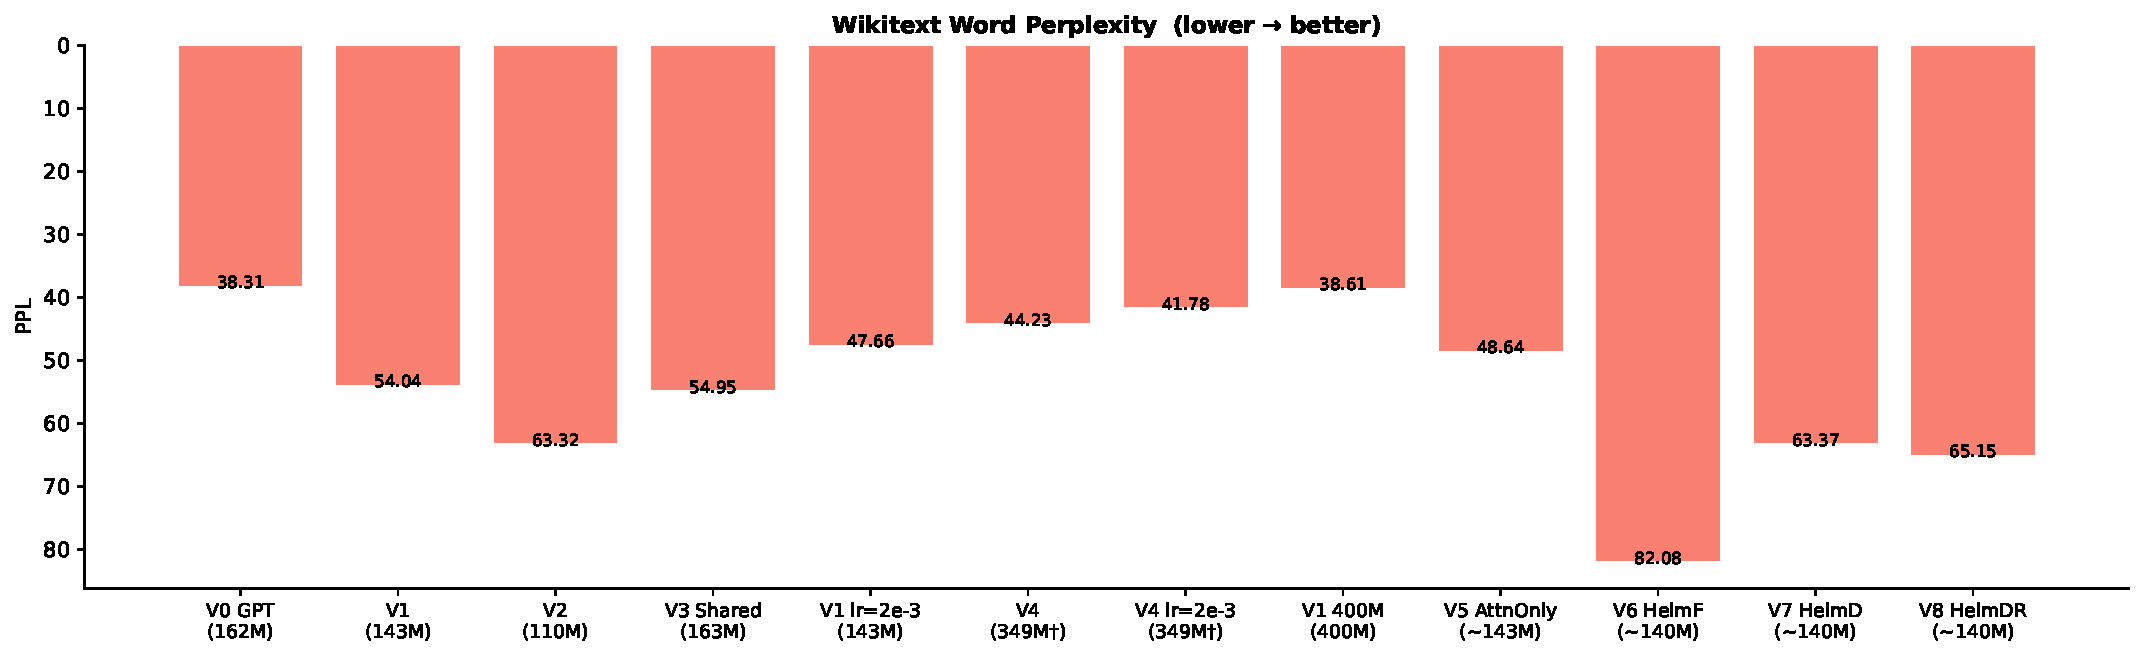
\includegraphics[width=\textwidth]{../results/multi-block-ablation/plots/wikitext_ppl.pdf}
    \caption{WikiText word perplexity (lower is better).}
    \label{fig:ppl}
  \end{subfigure}
  \hfill
  \begin{subfigure}[b]{0.48\textwidth}
    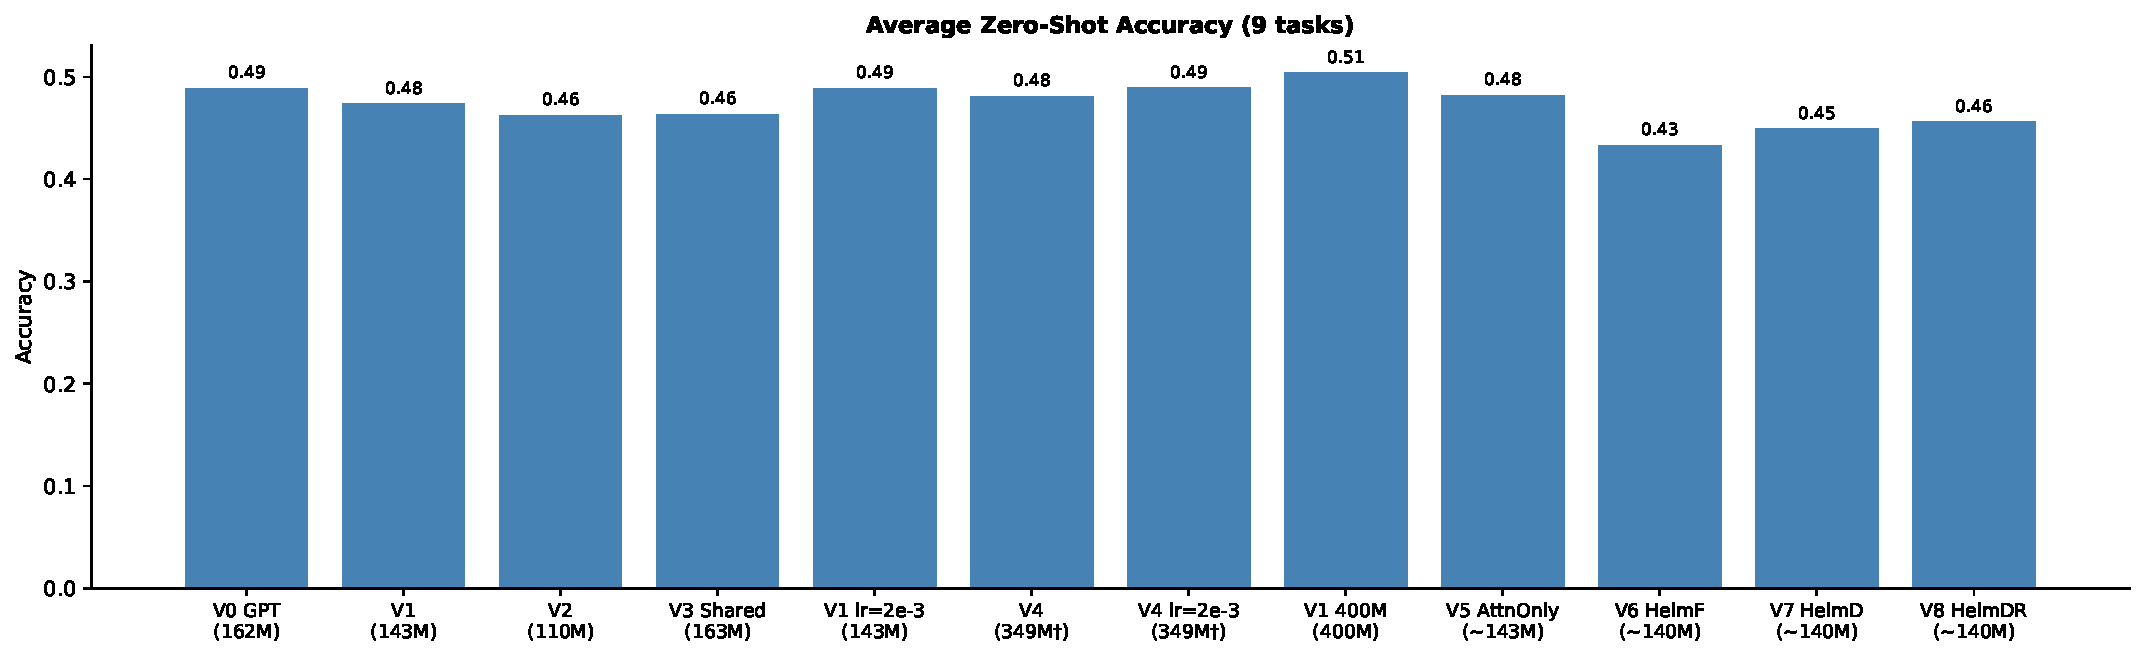
\includegraphics[width=\textwidth]{../results/multi-block-ablation/plots/avg_zeroshot_acc.pdf}
    \caption{Average zero-shot accuracy (9 tasks).}
    \label{fig:avg_acc}
  \end{subfigure}
  \caption{Summary metrics across model variants.  V0 GPT leads on both axes;
    V1 at lr=2e-3 substantially closes the gap over V1 at lr=3e-4.}
  \label{fig:summary}
\end{figure}

\begin{figure}[h]
  \centering
  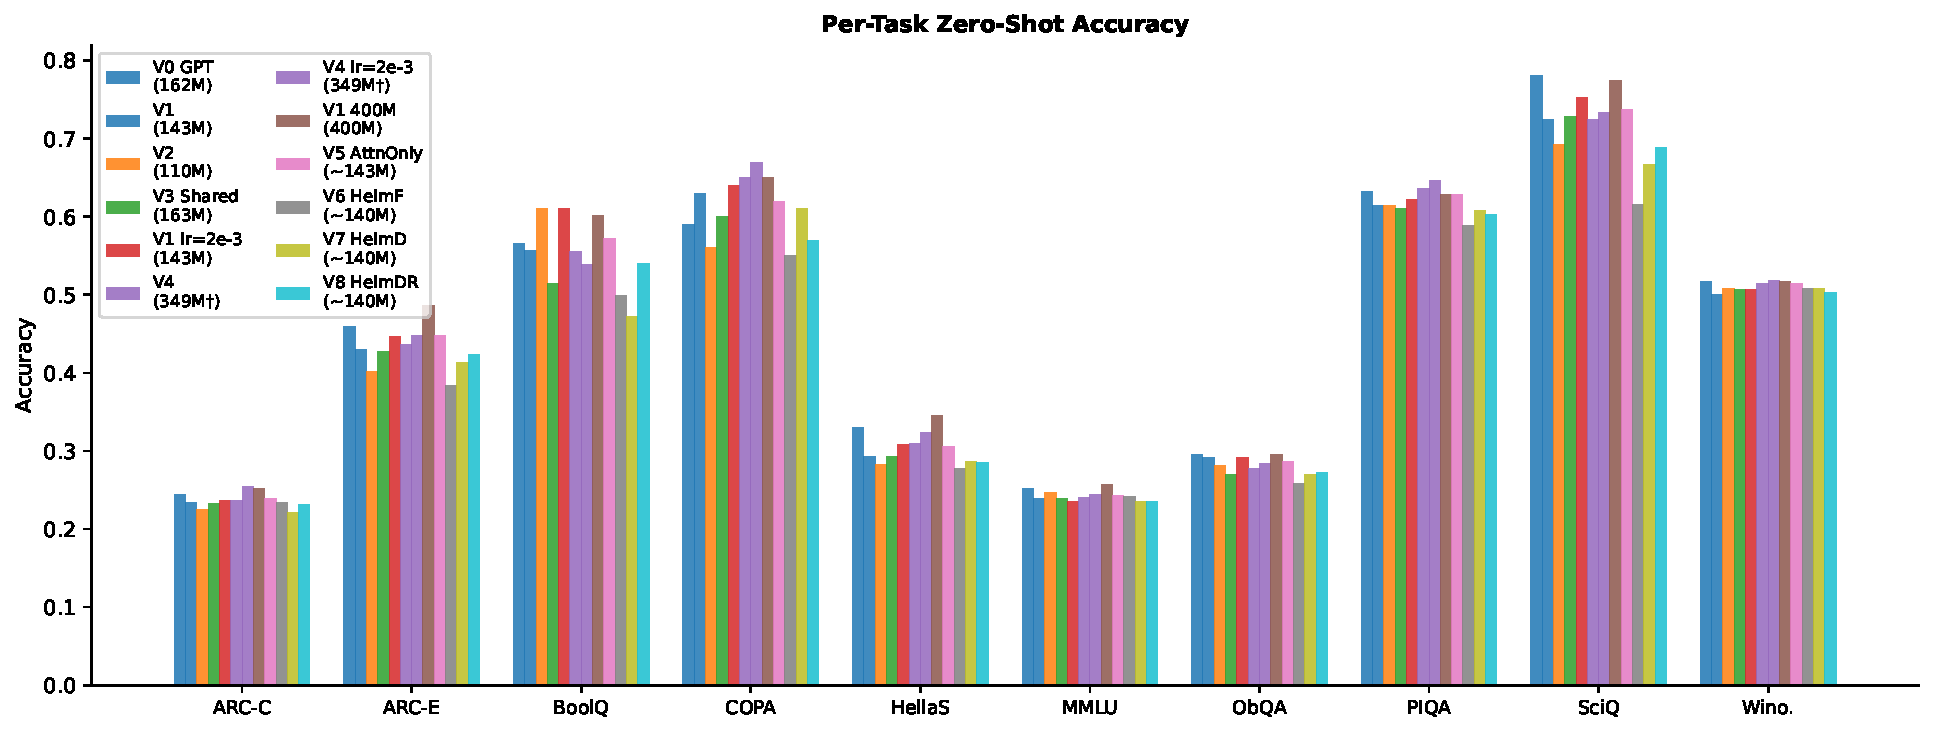
\includegraphics[width=0.95\textwidth]{../results/multi-block-ablation/plots/per_task_breakdown.pdf}
  \caption{Per-task zero-shot accuracy for all evaluated variants.
    Energy models trail GPT on most tasks but lead on BoolQ and COPA.}
  \label{fig:per_task}
\end{figure}

\begin{figure}[h]
  \centering
  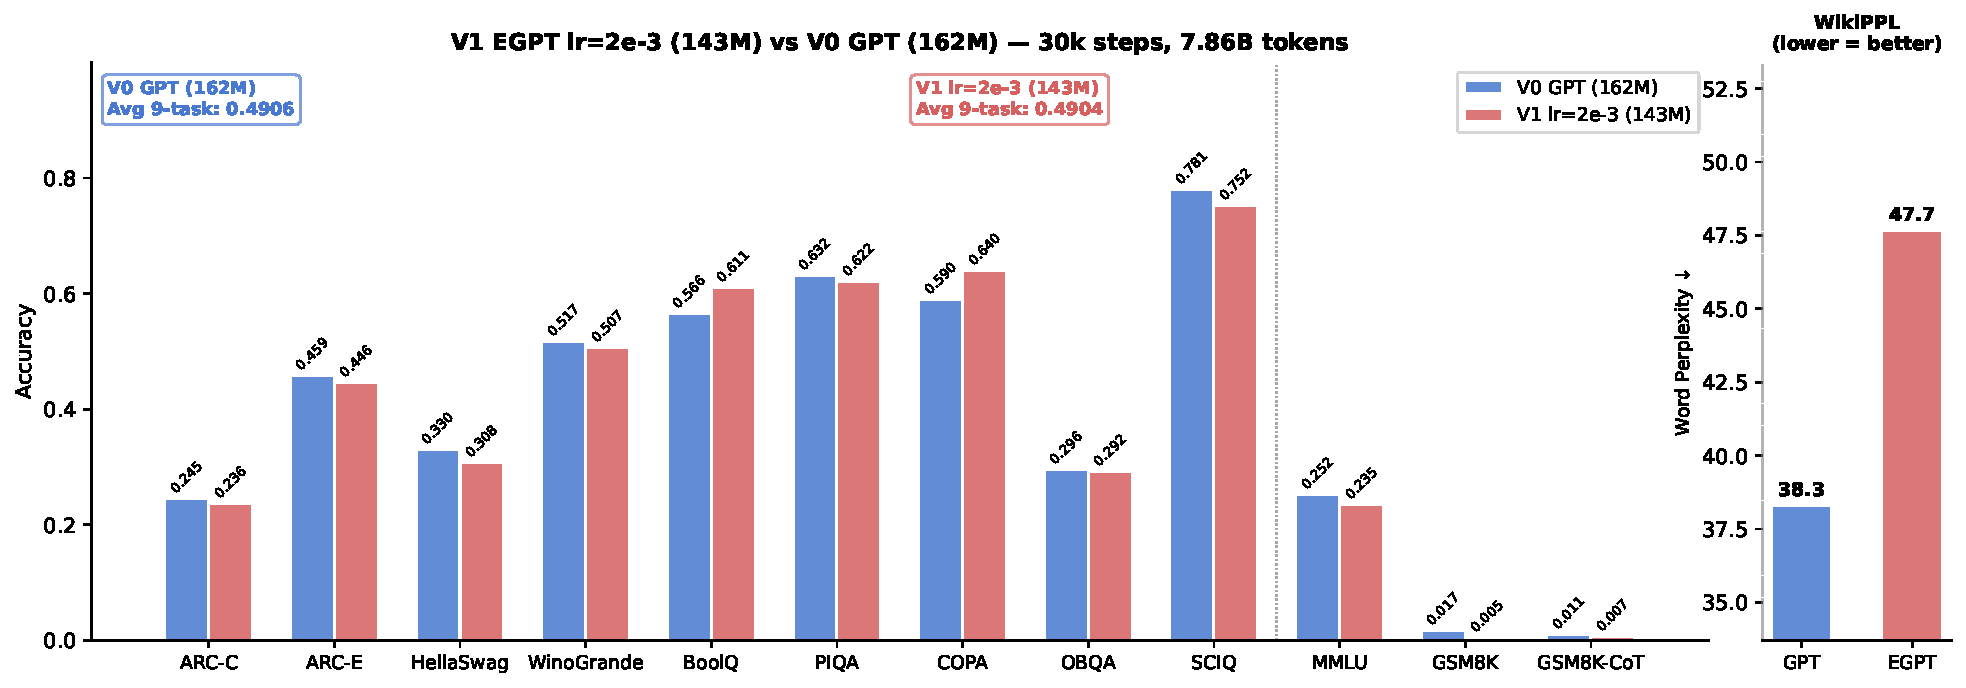
\includegraphics[width=\textwidth]{../results/multi-block-ablation/plots/v1_vs_gpt.pdf}
  \caption{Direct iso-param/iso-compute comparison: V1 EGPT lr=2e-3 (143M) vs.\
    V0 GPT (162M) at 30k steps (7.86B tokens).
    Average zero-shot: EGPT 0.490 vs.\ GPT 0.491 ($\Delta = -0.0002$, virtually tied).
    EGPT leads only on BoolQ (+0.045) and COPA (+0.050).
    GPT leads substantially on perplexity (38.3 vs.\ 47.7) and on GSM8K.}
  \label{fig:v1_vs_gpt}
\end{figure}

\paragraph{Key observations.}
\begin{itemize}
  \item \textbf{EGPT is significantly less compute-efficient than GPT.}
    V1 400M (400M params, $d=1024$, 24 layers) uses \textbf{4.4$\times$ more FLOPs per
    token} than V0 GPT (162M, $d=768$, 12 layers): the extra depth, wider $d$, and two
    additional $d{\times}d$ projection matmuls per block add up to 755M vs.\ 170M
    FLOPs/token.\footnote{FLOPs counted as $2\times$ matmul operations per token, excluding
    attention softmax and layer norms.}
    Despite this, V1 400M achieves only marginally better results (PPL 38.6 vs.\ 38.3,
    avg zero-shot 0.506 vs.\ 0.491).
    \emph{An iso-compute 400M GPT trained on the same tokens would be expected to
    substantially outperform both.}
  \item \textbf{Training loss alignment confirms the efficiency gap.}
    The 400M EGPT training loss curve closely tracked the 162M GPT loss curve on WandB,
    even though the two models differ by 4.4$\times$ in compute.
    Benchmarks confirm the tracking: EGPT at 4.4$\times$ the cost approximately equals GPT,
    i.e., EGPT's effective compute utilisation is roughly $1/4$ that of GPT at this scale.
  \item \textbf{At iso-param 160M scale, GPT leads on all metrics.}
    The best 160M EGPT variant (V1 lr=2e-3) nearly ties GPT on zero-shot (0.490 vs.\ 0.491)
    but trails on perplexity (47.7 vs.\ 38.3, a $-24\%$ gap).
    Higher LR (3e-4 $\to$ 2e-3) closes zero-shot but not perplexity.
  \item \textbf{V4 (349M, 20k steps) matches GPT zero-shot at yet higher cost.}
    V4 lr=2e-3 ties GPT on avg zero-shot (0.491) but uses $\sim$349M params and only 20k
    steps --- another data point confirming EGPT needs more parameters to reach GPT parity.
  \item \textbf{V3 shared backbone matches V1 distinct blocks} on perplexity (55.0 vs.\ 54.0)
    with far fewer unique parameters, indicating the recurrence contributes useful computation.
  \item \textbf{V2 (6 blocks $\times$ 2 iters) is the weakest} at 30k steps: fewer distinct
    blocks with repeated iterations does not compensate.
  \item \textbf{GSM8K near-zero for all EGPT variants.}
    GPT leads on both greedy (0.017) and CoT (0.011).  V1 400M reaches 0.007 greedy but
    only 0.003 CoT --- too small to benefit from chain-of-thought prompting.
\end{itemize}

%% ============================================================
\section{Curl--Gradient Analysis of Projection Matrices}
\label{sec:curl_grad}
%% ============================================================

\subsection{Helmholtz Decomposition}

For a square projection matrix $W \in \mathbb{R}^{d \times d}$:
\begin{align*}
  S = \frac{W + W^\top}{2} \quad \text{(symmetric, gradient component)}, \\
  A = \frac{W - W^\top}{2} \quad \text{(anti-symmetric, curl component)}.
\end{align*}
We define the \emph{curl-to-gradient ratio}:
\[
  \rho = \frac{\|A\|_F}{\|S\|_F}.
\]
$\rho > 1$ means curl dominates; $\rho < 1$ means gradient/dissipation dominates;
$\rho = 1$ corresponds to the balanced mid-point where $\|S\|_F = \|A\|_F$.
For a random matrix with i.i.d.\ entries, $\rho = 1$ exactly by symmetry.

\subsection{Per-layer Ratios}

We compute $\rho$ for each layer's $\mathrm{proj\_attn}$ and $\mathrm{proj\_mlp}$ in two
trained models: V1 at lr=2e-3 (30k steps, $d=768$) and V4 at lr=2e-3 (10k steps, $d=1152$).

\begin{figure}[h]
  \centering
  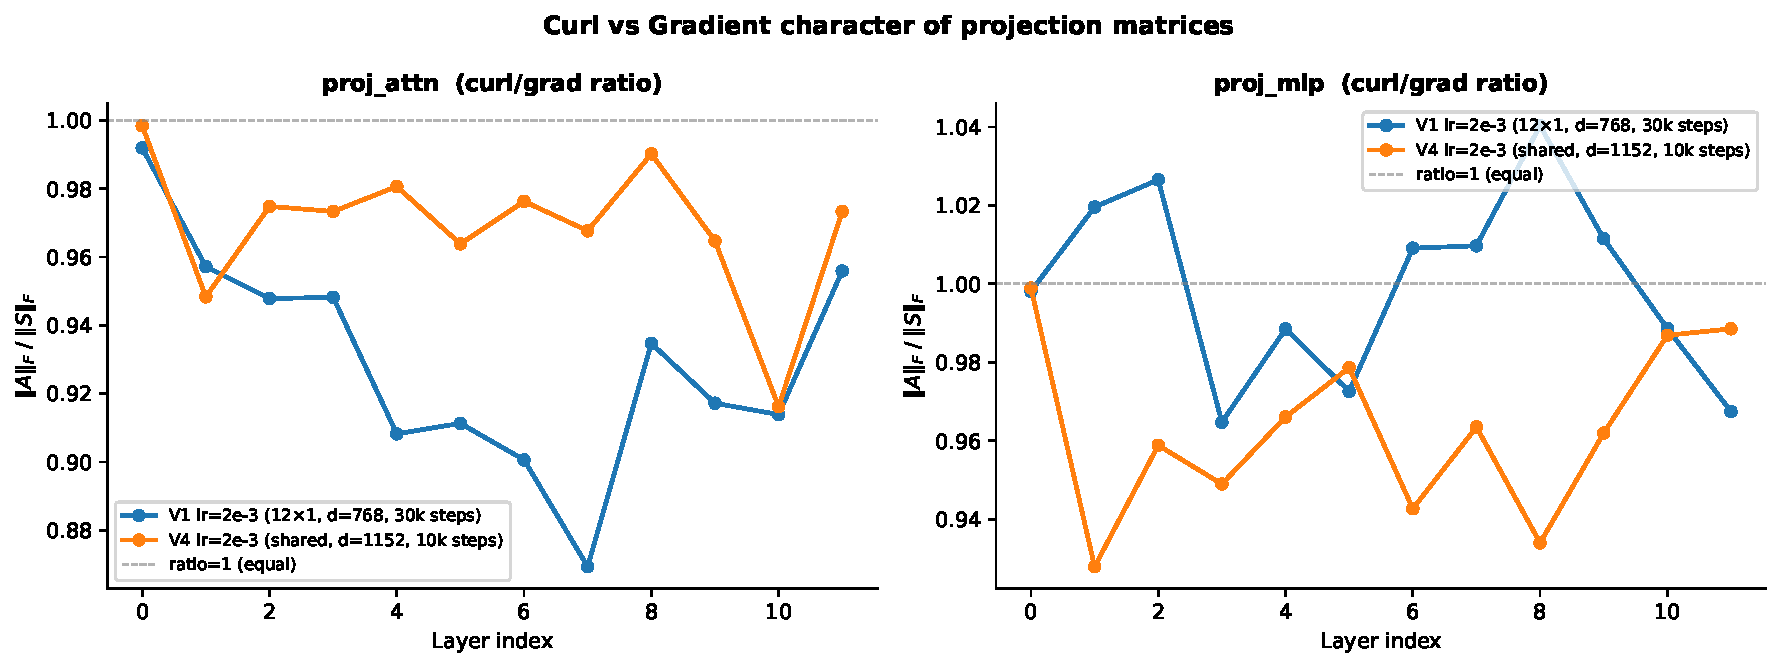
\includegraphics[width=0.92\textwidth]{../results/multi-block-ablation/plots/curl_grad_ratio.pdf}
  \caption{Per-layer curl-to-gradient ratio $\|A\|_F / \|S\|_F$ for
    $\mathrm{proj\_attn}$ (left) and $\mathrm{proj\_mlp}$ (right).
    The dashed line marks $\rho = 1$ (balanced).
    All layers across both models remain close to 1.}
  \label{fig:curl_grad}
\end{figure}

\paragraph{Results.}
\begin{itemize}
  \item \textbf{V1 lr=2e-3}: mean $\rho_{\mathrm{attn}} = 0.930$,
    mean $\rho_{\mathrm{mlp}} = 1.000$.
    The attention stream shows a mild gradient bias (slightly below 1), most pronounced
    at layer 7 ($\rho \approx 0.87$).  The MLP stream is almost perfectly balanced
    ($\rho \approx 1.0$ at every layer).
  \item \textbf{V4 lr=2e-3}: mean $\rho_{\mathrm{attn}} = 0.969$,
    mean $\rho_{\mathrm{mlp}} = 0.963$.
    Both streams are uniformly close to 1 ($\rho \in [0.93, 0.99]$ across all layers),
    with no systematic depth trend.
\end{itemize}

\paragraph{Interpretation.}
Both models converge to a near-balanced Helmholtz decomposition, consistent with the
prior finding on the 410M hybrid model that the projection matrices learn
$\|S\|_F \approx \|A\|_F$ regardless of initialisation.
This balance is not an artefact of random initialisation: for random Gaussian matrices
the ratio is exactly 1, but the proximity to 1 after training is maintained across 30k
steps and across two different model sizes and learning rates.
The slight gradient bias ($\rho < 1$) in V1's attention stream may reflect an inductive
bias toward dissipation in the attention pathway, consistent with the observation from
per-layer alpha sweeps that early layers are more sensitive to excess curl.

%% ============================================================
\section{Layer Similarity Analysis: Do EGPT Layers Share the Same Energy?}
%% ============================================================

A central claim of the EGPT design is that each block performs an iterative
gradient step on a \emph{shared} energy landscape.
If true, we expect the pre-projection activations
$\mathrm{attn\_out}^{(i)} = \mathrm{attn}(\mathrm{LN}(x^{(i)}))$ and
$\mathrm{ffwd\_out}^{(i)} = \mathrm{ffwd}(\mathrm{LN}(x^{(i)}))$
--- which we interpret as the gradient signal $\nabla_x E$ at each recurrence step ---
to be \emph{more similar across layers} than in a standard GPT of the same size.
The projection matrices ($\mathrm{proj\_attn}$, $\mathrm{proj\_mlp}$) act as the
\emph{policy}: step size, direction mixing, and exploration--exploitation balance,
which may differ per layer even if the gradient signal is shared.

\subsection{Setup}

We pass a 512-token WikiText prefill through three models ---
V1 EGPT lr=2e-3 (trained), V0 GPT (trained), and a randomly-initialised V1 EGPT
(same architecture, untrained) --- and capture four activation tensors per layer:

\begin{itemize}
  \item \textbf{h\_out}: the residual stream state after the full block update.
  \item \textbf{attn\_out}: pre-projection attention output, i.e.\ $\mathrm{attn}(\mathrm{LN}(x))$.
    This is the \emph{attention gradient signal} before the policy is applied.
  \item \textbf{ffwd\_out}: pre-projection FFN output, i.e.\ $\mathrm{ffwd}(\mathrm{LN}(x))$.
    This is the \emph{FFN gradient signal}.
  \item \textbf{update} ($\Delta x$): the delta applied to the residual,
    $x^{(i+1)} - x^{(i)}$ (negative for EGPT, positive for GPT).
    This captures the combined policy output.
\end{itemize}

We report two metrics for the $12 \times 12$ inter-layer similarity matrix:
\textbf{Linear CKA} (Centered Kernel Alignment, geometry-aware and scale-invariant)
and \textbf{mean cosine similarity} (directional alignment across token positions).

\subsection{Results and Interpretation}

\begin{table}[h]
\centering
\caption{Mean off-diagonal inter-layer similarity.
  Random = randomly-initialised V1 EGPT (untrained baseline).}
\label{tab:layer_sim}
\small
\setlength{\tabcolsep}{5pt}
\begin{tabular}{llccc}
\toprule
\textbf{Component} & \textbf{Metric} & \textbf{V1 EGPT} & \textbf{V0 GPT} & \textbf{Random} \\
\midrule
h\_out (residual)     & CKA    & 0.663 & 0.572 & 0.952 \\
                      & Cosine & \textbf{0.764} & 0.612 & 0.670 \\
\midrule
attn\_out (grad$_E$)  & CKA    & 0.463 & 0.326 & 0.961 \\
                      & Cosine & \textbf{0.176} & 0.119 & 0.006 \\
\midrule
ffwd\_out (grad$_E$)  & CKA    & 0.513 & 0.367 & 0.891 \\
                      & Cosine & $-0.000$ & 0.078 & $-0.002$ \\
\midrule
update ($\Delta x$)   & CKA    & 0.380 & \textbf{0.383} & 0.849 \\
                      & Cosine & 0.022 & \textbf{0.085} & $-0.001$ \\
\bottomrule
\end{tabular}
\end{table}

\begin{figure}[h]
  \centering
  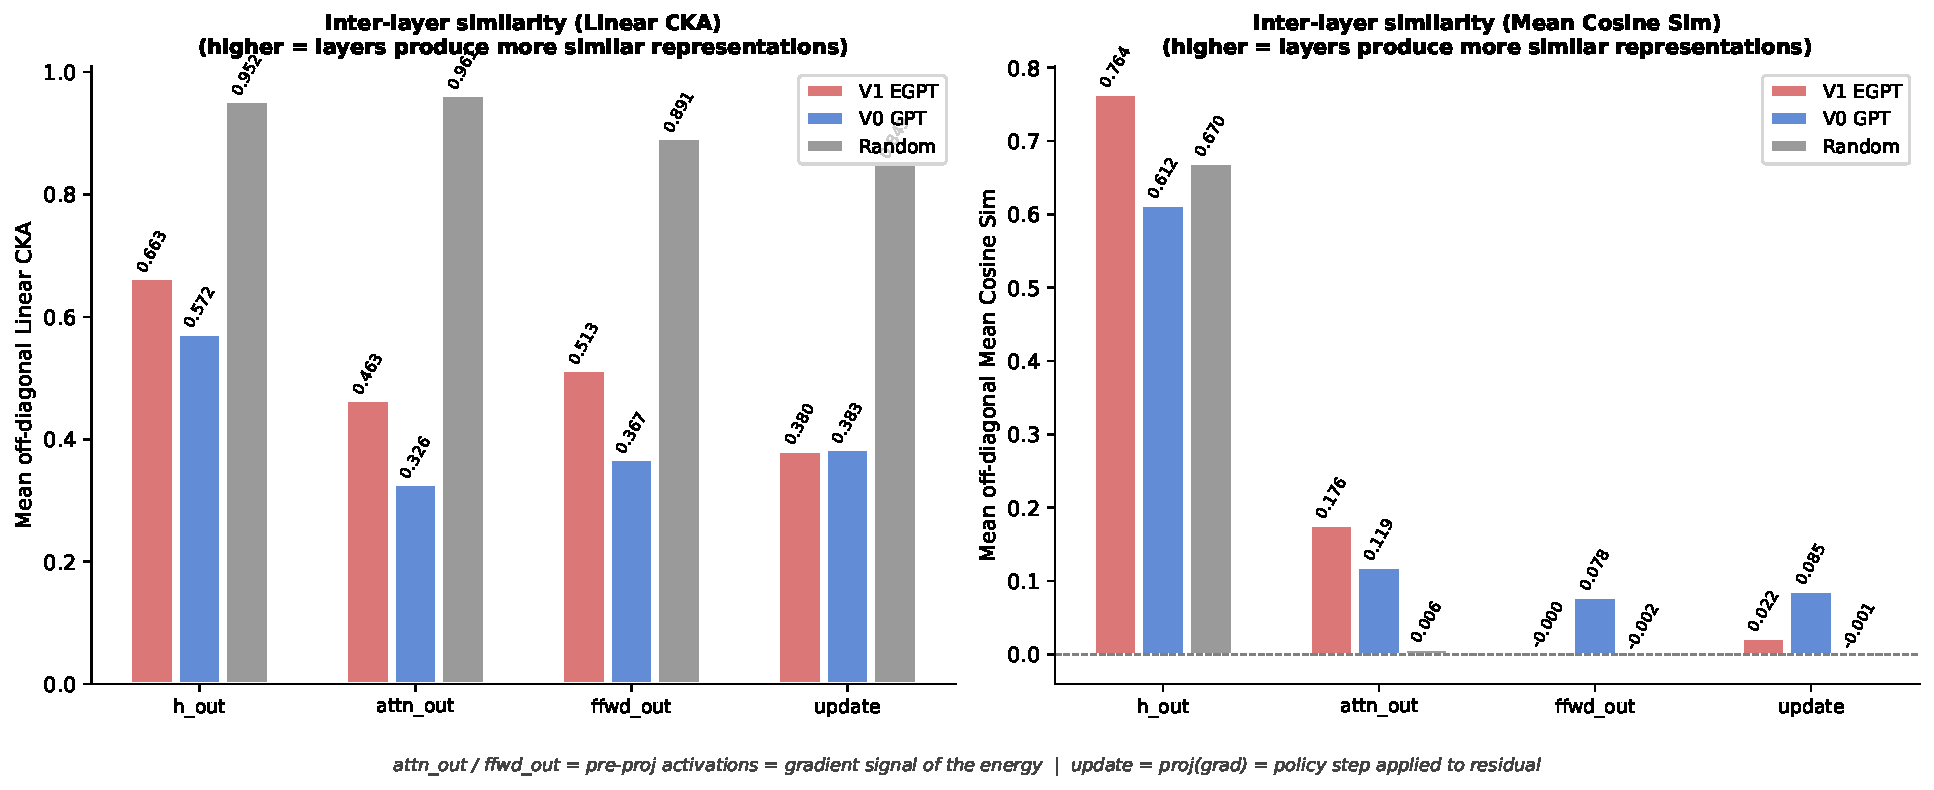
\includegraphics[width=\textwidth]{../results/multi-block-ablation/plots/layer_sim_summary.pdf}
  \caption{Mean off-diagonal inter-layer similarity (CKA and cosine) for each
    activation component across three models.  Random = untrained baseline.}
  \label{fig:layer_sim_summary}
\end{figure}

\begin{figure}[h]
  \centering
  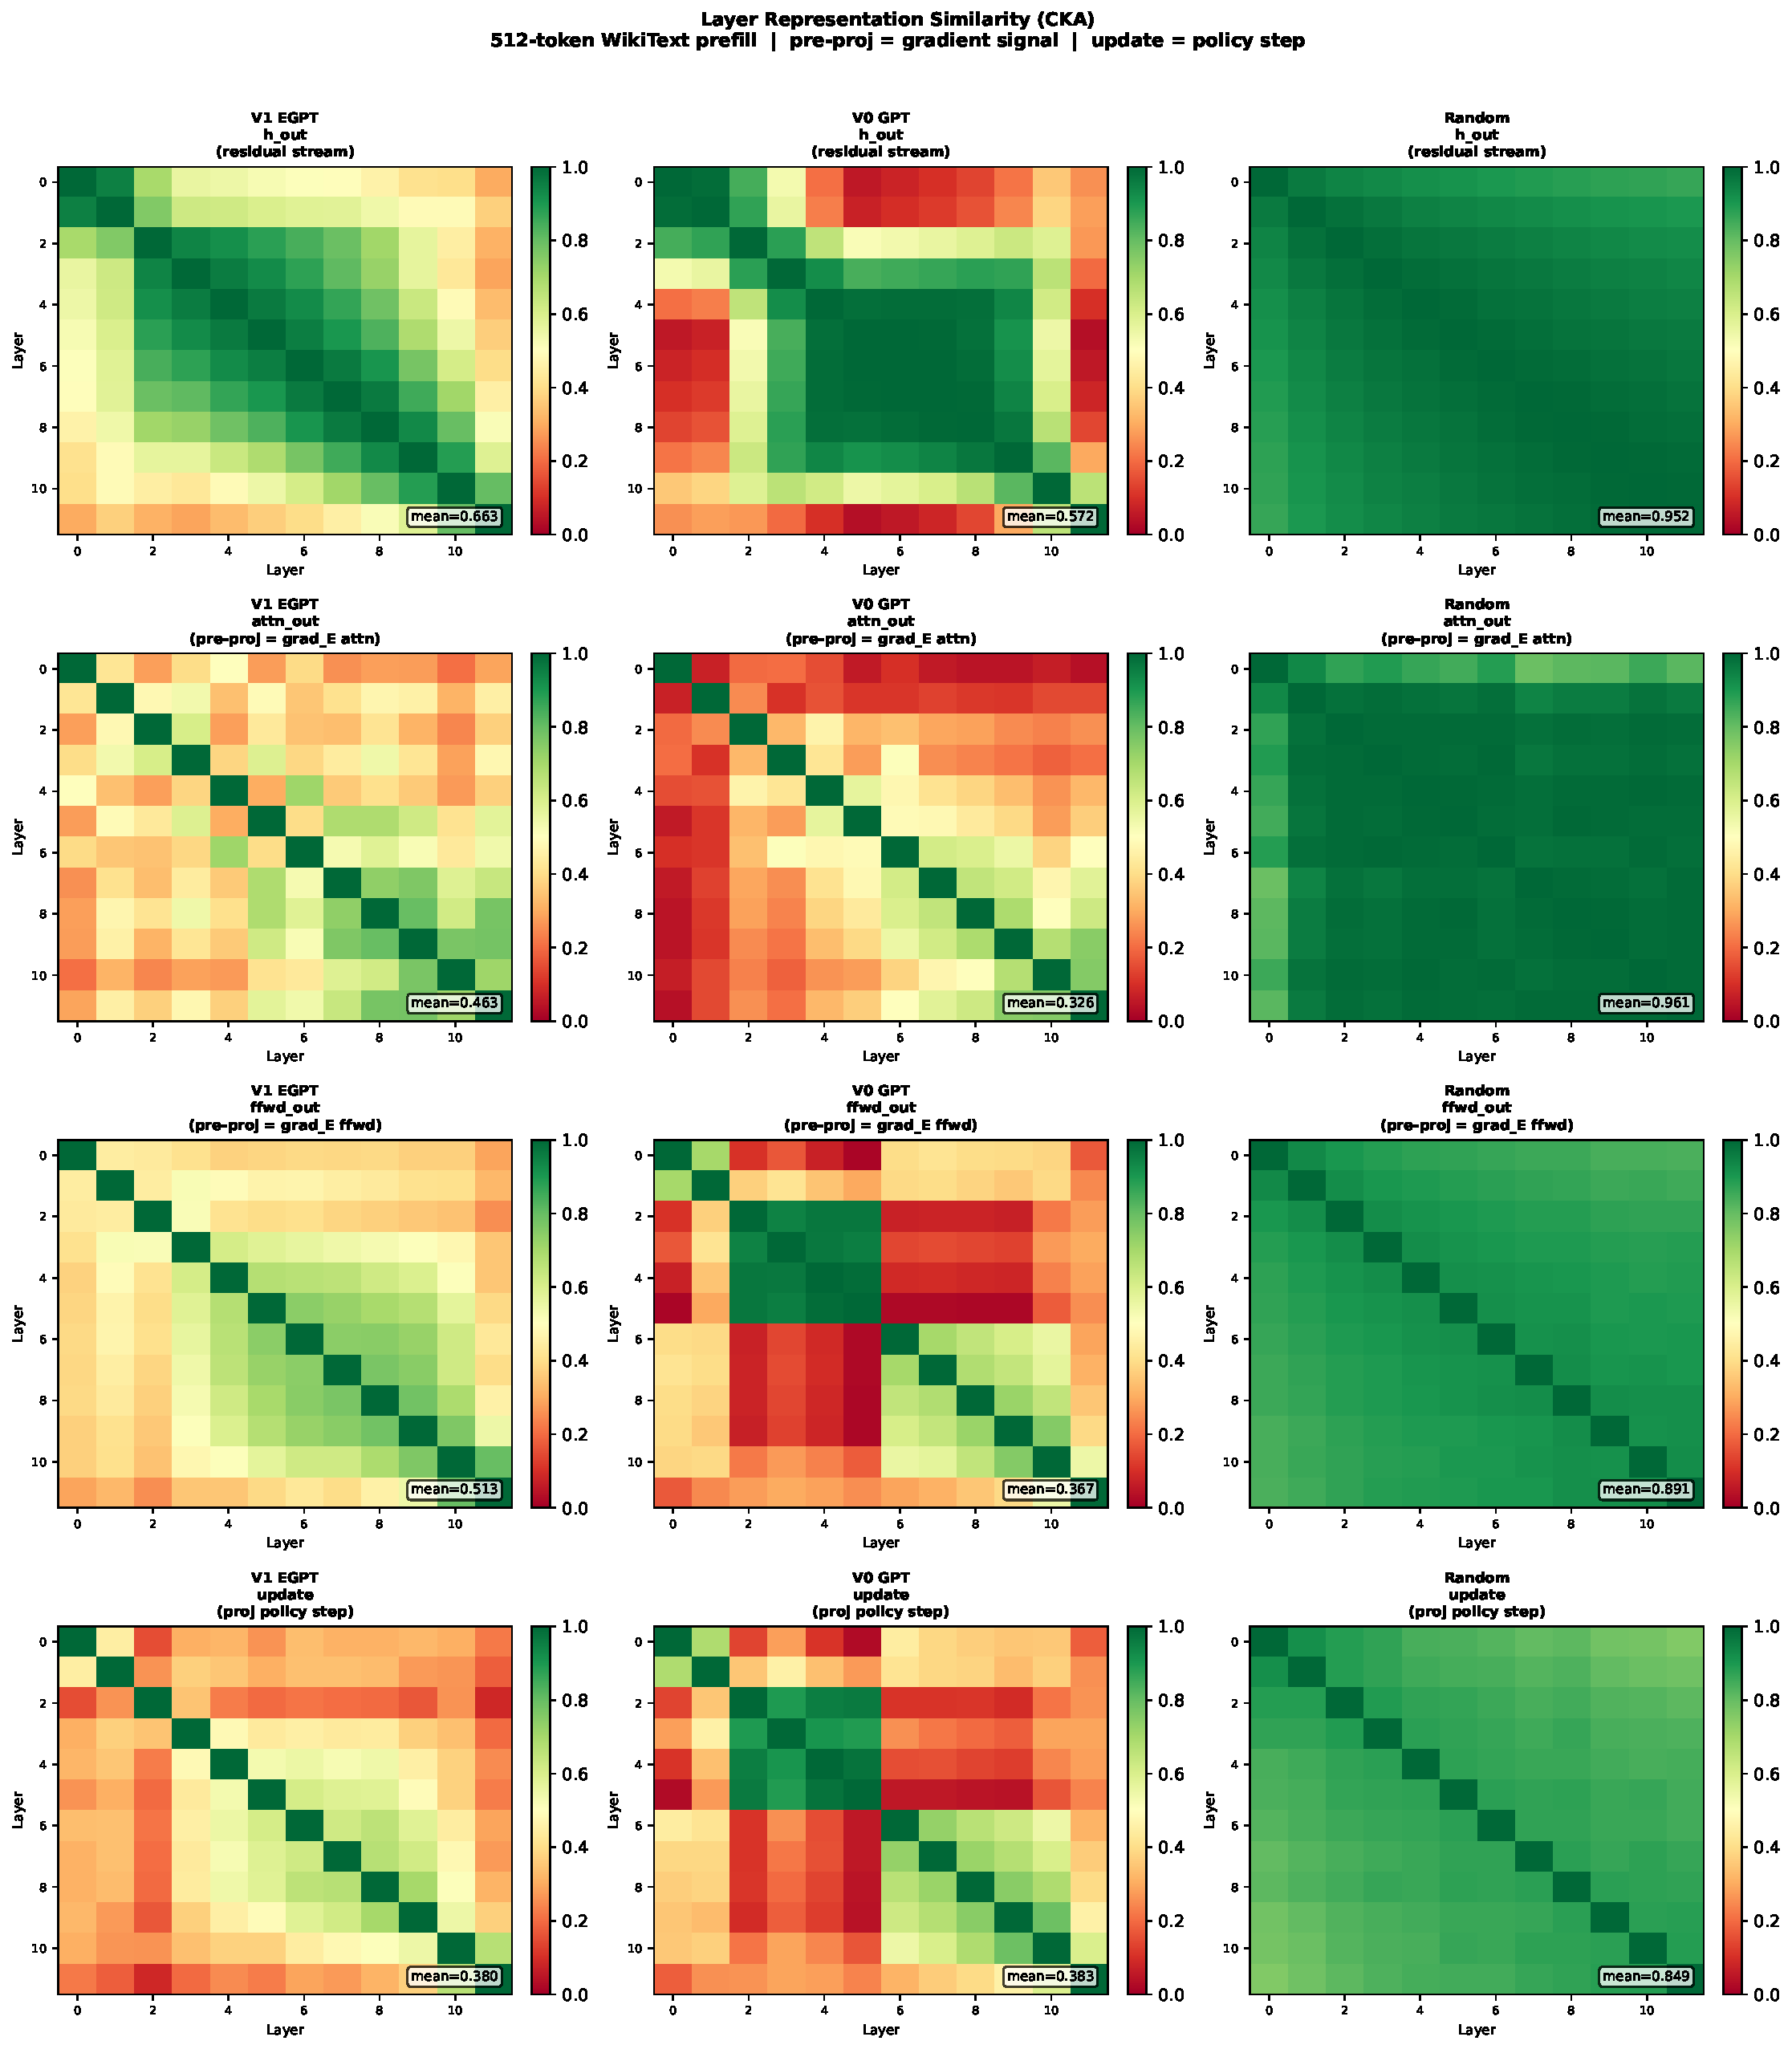
\includegraphics[width=\textwidth]{../results/multi-block-ablation/plots/layer_sim_cka.pdf}
  \caption{Full $12\!\times\!12$ inter-layer Linear CKA matrices for each activation
    component, across V1 EGPT lr=2e-3 (trained), V0 GPT (trained), and random-init
    V1 EGPT.  The random model attains the highest CKA (0.85--0.96) because all layers
    receive the same embedded input through the residual stream; training specialises layers
    and \emph{reduces} CKA.  CKA is therefore dominated by input geometry and is a
    poor probe of the shared-energy hypothesis.}
  \label{fig:layer_sim_cka}
\end{figure}

\begin{figure}[h]
  \centering
  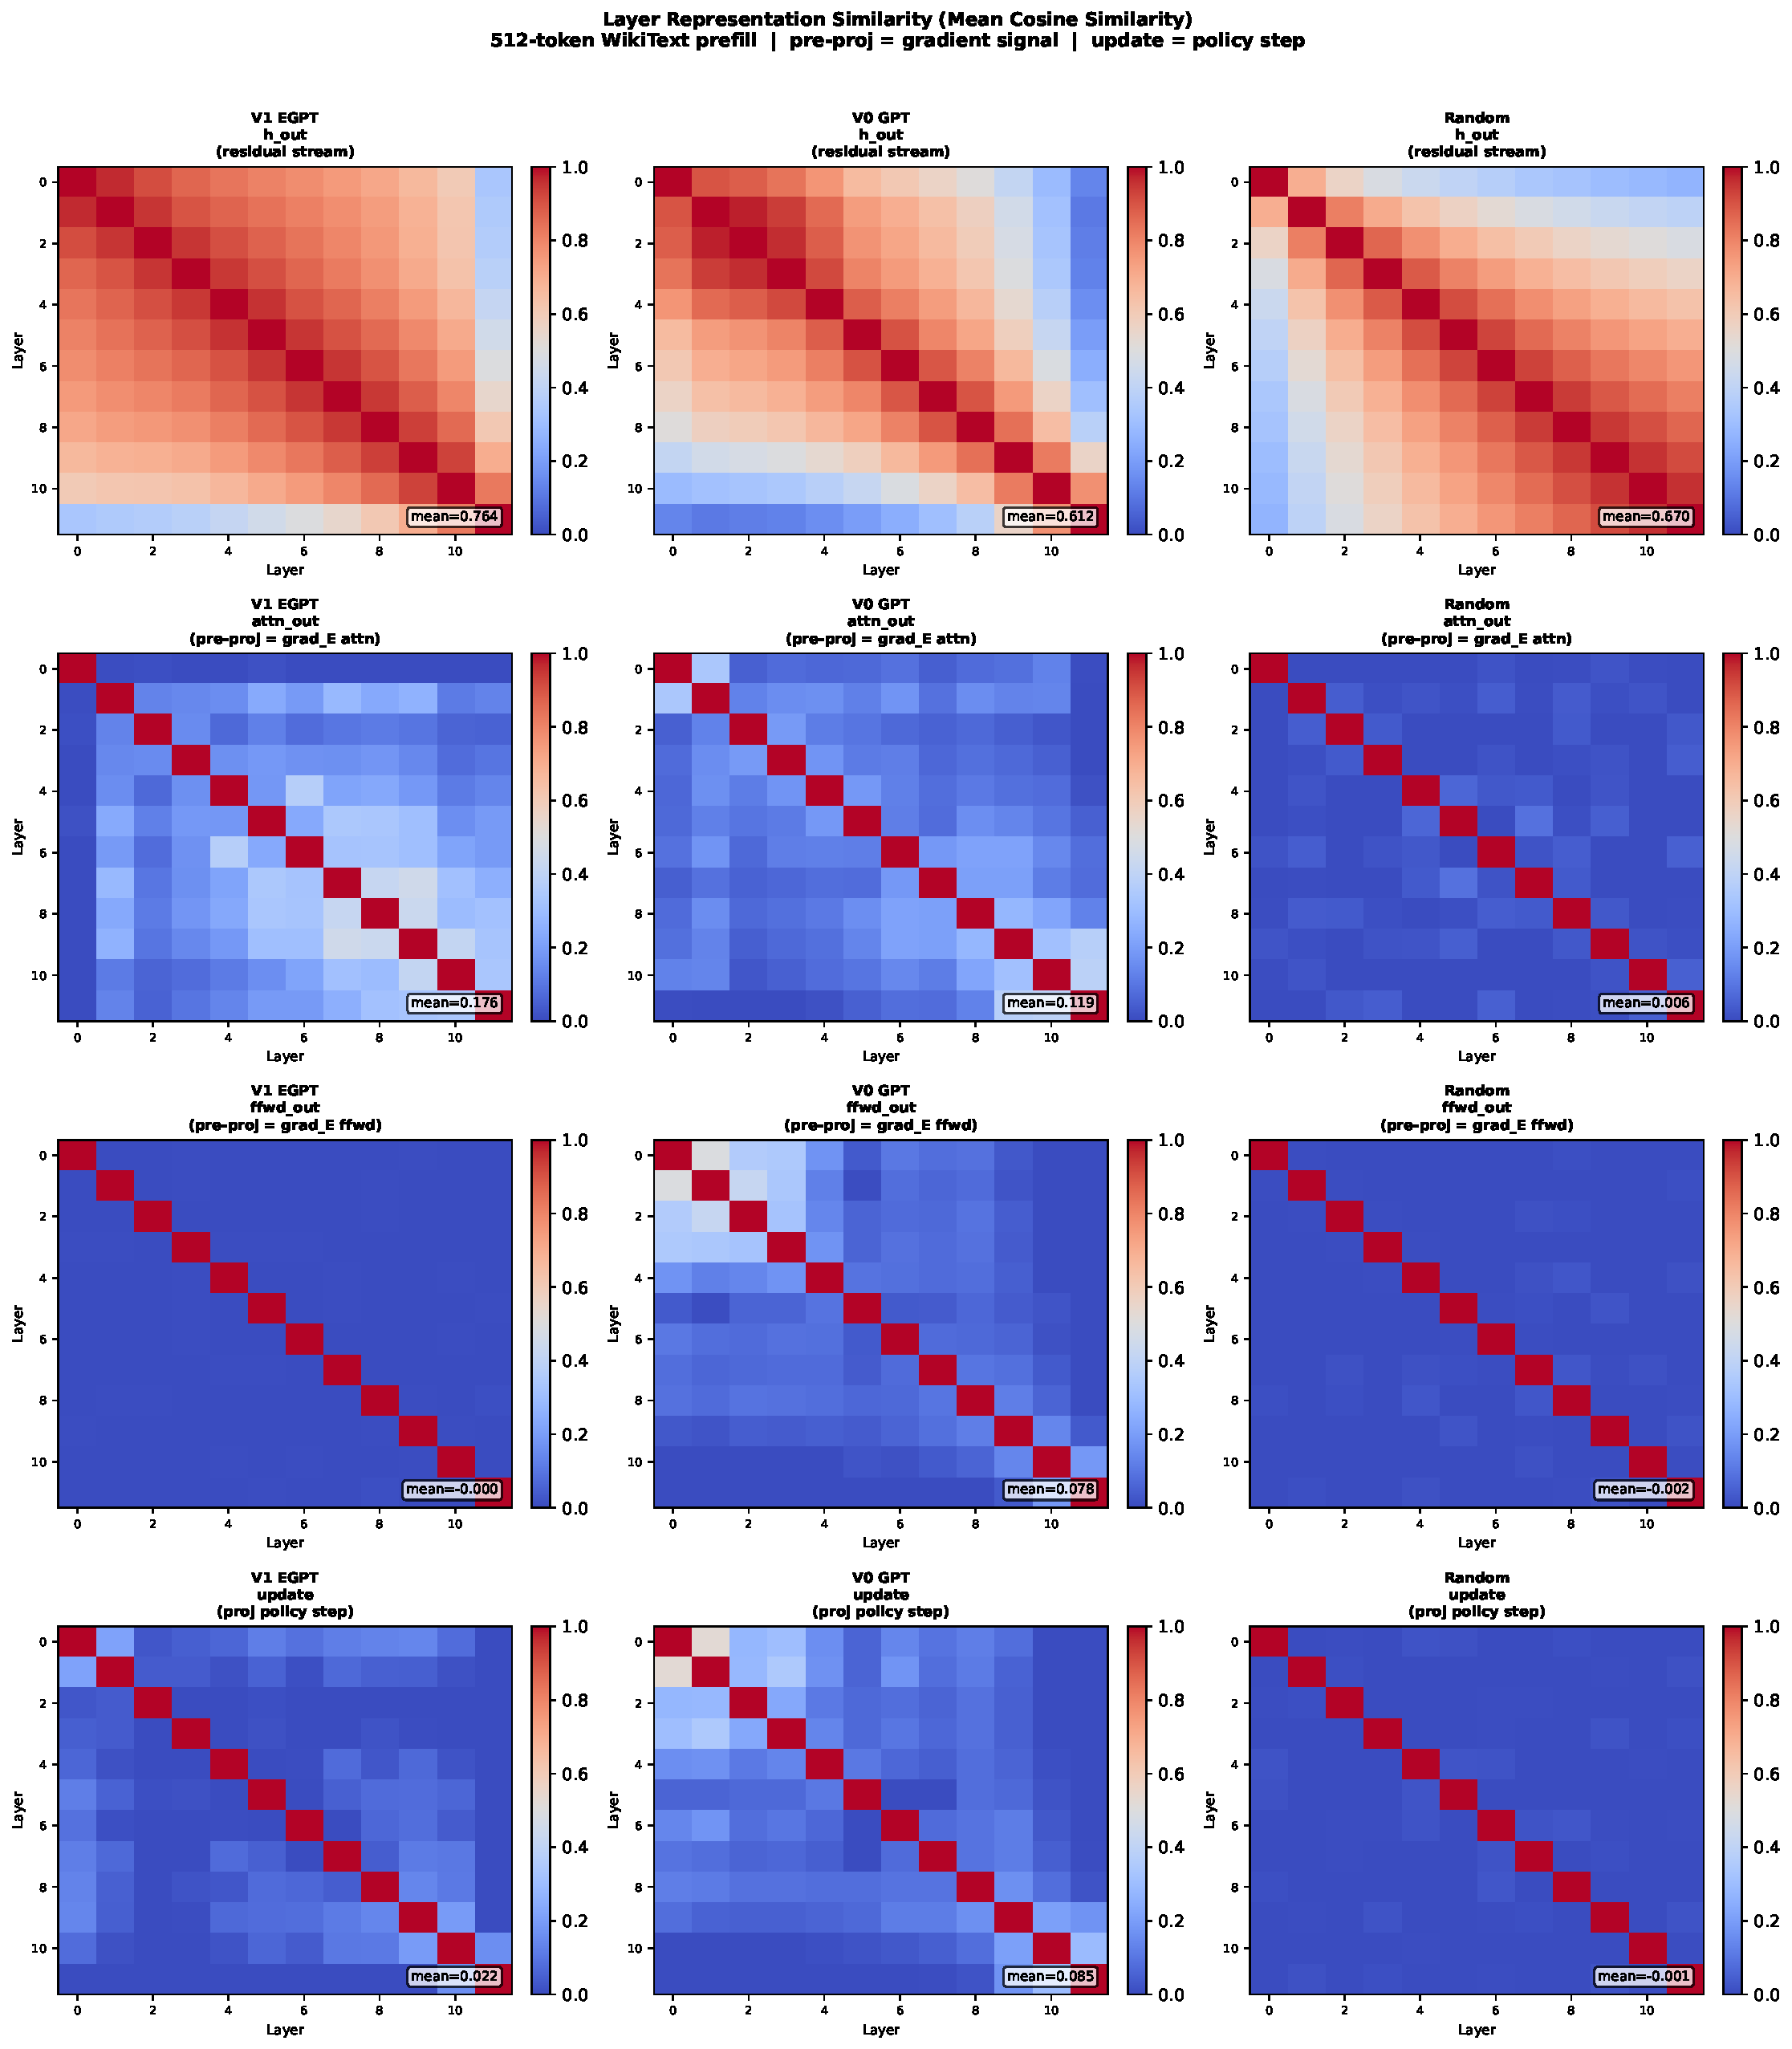
\includegraphics[width=\textwidth]{../results/multi-block-ablation/plots/layer_sim_cosine.pdf}
  \caption{Full $12\!\times\!12$ inter-layer mean cosine similarity matrices.
    The random baseline is near zero for all components (confirming no spurious signal),
    making cosine similarity a reliable probe of genuine cross-layer alignment.
    The attn\_out panel (gradient signal) shows the highest off-diagonal values for
    V1 EGPT (0.176), exceeding GPT (0.119), consistent with shared attention-energy structure.
    The ffwd\_out panel is near zero for EGPT, suggesting the FFN gradient is not shared
    across layers.}
  \label{fig:layer_sim_cosine}
\end{figure}

\paragraph{CKA is dominated by input geometry, not model structure.}
Strikingly, the random-init model achieves the \emph{highest} CKA across all components
(0.85--0.96), far above both trained models.
This occurs because all layers receive the same embedded input through the residual connection,
and random linear projections of the same input preserve similar Gram matrices.
Training \emph{reduces} CKA by specialising each layer's representation.
CKA is therefore a poor tool for testing the shared-energy hypothesis in this setting;
it primarily reflects how much each layer has diverged from the input.

\paragraph{Cosine similarity reveals genuine cross-layer structure.}
The random baseline has near-zero cosine similarity for all sub-module outputs
(0.006 for attn, $-0.002$ for ffwd, $-0.001$ for update), confirming that
cosine similarity correctly identifies the absence of cross-layer directional alignment
in untrained models.

\begin{itemize}
  \item \textbf{attn\_out (attention gradient): EGPT $>$ GPT $\gg$ random.}
    V1 EGPT shows cosine 0.176 across layers vs.\ 0.119 for GPT and 0.006 for random.
    The attention pre-projection outputs are \emph{more directionally aligned} across
    EGPT blocks than in GPT, and far above the random baseline.
    This is the strongest positive evidence that EGPT layers may be computing
    gradient signals of a shared energy function.

  \item \textbf{ffwd\_out (FFN gradient): near zero for all models.}
    Despite higher CKA (0.51), the FFN pre-projection cosine is $-0.000$ for EGPT,
    comparable to random ($-0.002$) and \emph{lower} than GPT (0.078).
    The FFN outputs are not directionally aligned across layers in EGPT.
    This weakens the shared-energy interpretation: if all layers optimised the same
    energy via FFN, we would expect positive cosine similarity.

  \item \textbf{update ($\Delta x$): GPT $>$ EGPT $\approx$ random.}
    The full policy-applied step is \emph{less} cross-layer aligned in EGPT (0.022)
    than in GPT (0.085), and both are above random ($-0.001$).
    The projection ``policy'' in EGPT does not produce more coherent cross-layer steps;
    if anything, GPT's residual additions are slightly more consistent in direction.

  \item \textbf{h\_out (residual stream): EGPT $>$ random $>$ GPT.}
    EGPT's residual stream cosine (0.764) is notably higher than GPT's (0.612) and
    even above the random baseline (0.670).
    This could reflect EGPT's subtractive update keeping the residual stream near a
    common attractor --- consistent with convergent gradient descent on a fixed energy ---
    rather than the progressive accumulation of information that characterises GPT.
\end{itemize}

\paragraph{Summary.}
The evidence for a shared energy across EGPT layers is mixed.
The attention pre-projection cosine similarity is above both GPT and random,
consistent with the shared-energy hypothesis for the attention stream.
The FFN pre-projection, however, shows no such alignment, and the policy-applied
updates ($\Delta x$) are less coherent in EGPT than in GPT.
The high residual-stream cosine similarity is suggestive of attractor-like dynamics
but is not conclusive without causal intervention experiments.
Overall, the layer similarity analysis motivates a more careful per-component study,
particularly of whether the attention stream alone carries the shared energy structure.

\paragraph{Consecutive-layer similarity reveals monotonic attention convergence in EGPT.}
Figure~\ref{fig:consecutive_layer_sim} plots $\cos(\text{attn\_out}_i, \text{attn\_out}_{i+1})$
and $\cos(\text{ffwd\_out}_i, \text{ffwd\_out}_{i+1})$ for adjacent block pairs $i \to i+1$.

\begin{figure}[h]
  \centering
  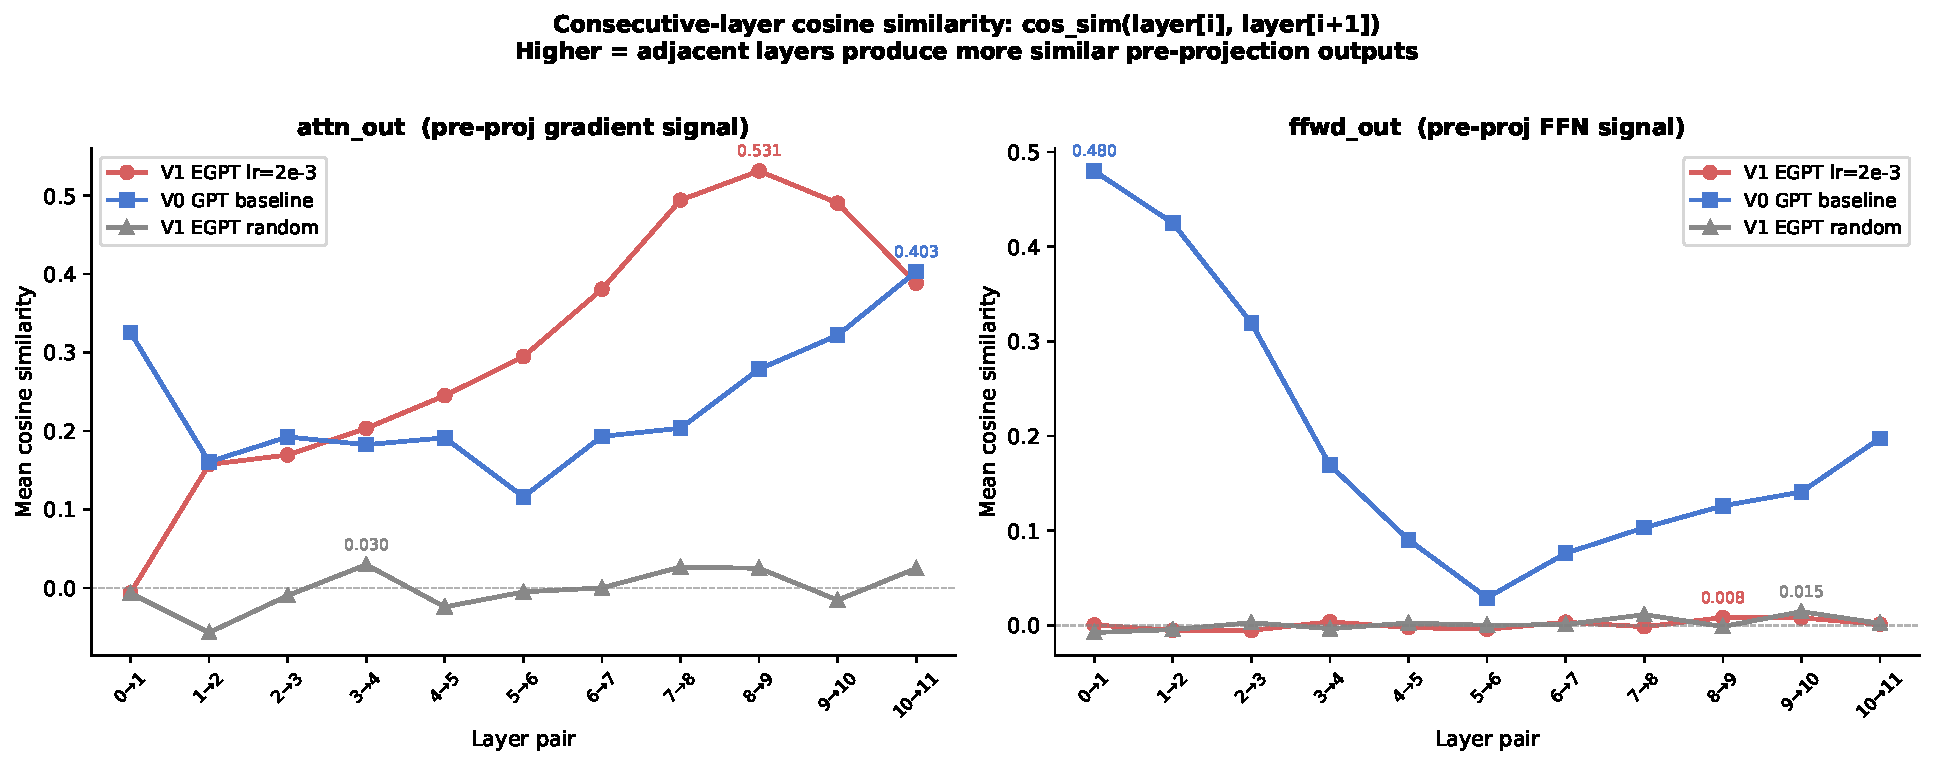
\includegraphics[width=\textwidth]{../results/multi-block-ablation/plots/consecutive_layer_sim.pdf}
  \caption{Consecutive-layer cosine similarity $\cos(\text{layer}_i, \text{layer}_{i+1})$ for
    attention pre-projection outputs (left) and FFN pre-projection outputs (right).
    V1 EGPT attention similarity rises monotonically from near 0 (early layers) to 0.53
    (layers 8--9), far above GPT ($\le 0.40$) and random ($\approx 0$).
    EGPT FFN similarity is near zero throughout, confirming the cross-layer average cosine
    captures only the attention stream structure.}
  \label{fig:consecutive_layer_sim}
\end{figure}

For \textbf{attn\_out}, V1 EGPT shows a striking monotonic increase: near zero at layers 0--1,
rising to a peak of 0.531 at layers 8--9, then declining slightly to 0.388 at 10--11.
GPT shows moderate values (0.12--0.40) with no clear trend.
The random baseline is $\approx 0$ throughout, confirming the EGPT pattern is learned.
This suggests the \emph{later} EGPT attention layers are computing nearly identical directions ---
strong evidence that they share a common gradient field.
Layers 6--10 (cosine $\ge 0.38$) are candidates for weight-sharing or averaging without
significant representation loss.

For \textbf{ffwd\_out}, EGPT is consistently near zero ($|r| < 0.01$) at all pairs,
while GPT starts at 0.48 and decays across depth.
FFN output norms in EGPT are healthy (mean L2 $\approx 8$--43), so the near-zero
cosine is not a dead-neuron artefact but genuine directional diversity:
EGPT's subtractive updates cause the residual stream $h$ to vary substantially between
adjacent layers, so the FFN sees different inputs and produces orthogonal outputs.

\paragraph{Layer merging: weight averaging is lossy and alignment does not help.}
To test whether high consecutive-layer cosine similarity implies mergeable weights,
we performed a systematic layer-merge PPL analysis.
For each candidate group of adjacent blocks, we averaged only the attention weights
(W$_Q$, W$_K$; FFN weights were not merged due to near-zero consecutive cosine similarity)
and dropped the redundant blocks, then measured WikiText-2 PPL immediately without retraining.

Figure~\ref{fig:layer_merge_ppl} shows the results.
Even the best single-pair merge (layers 7--8, the pair with second-highest attention cosine similarity)
increases PPL by 38\% (57.51 → 79.25).
Merging three blocks (7--9) costs 229\%; merging four (6--9) costs 488\%.
The pattern is not monotone with cosine similarity: pair (8,9) has the \emph{highest} consecutive
cosine (0.531) but the \emph{worst} single-pair PPL (+74\%), suggesting the output-space
similarity is decoupled from weight-space proximity.

\begin{figure}[h]
  \centering
  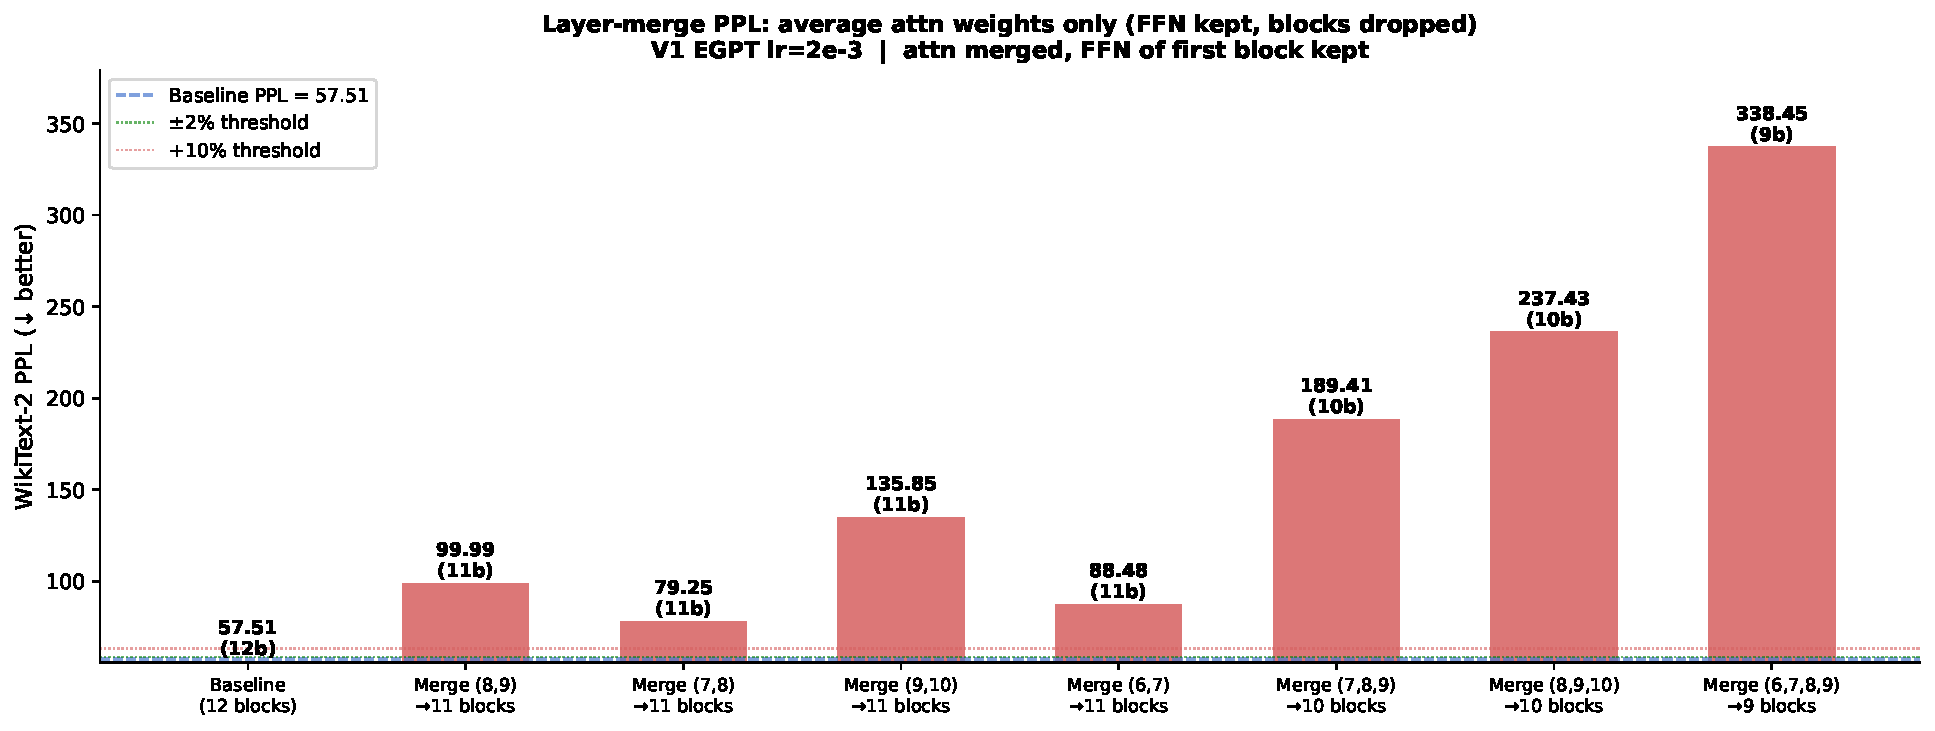
\includegraphics[width=\textwidth]{../results/multi-block-ablation/plots/layer_merge_ppl.pdf}
  \caption{WikiText-2 PPL for naive weight-averaged layer merges (attn only, FFN kept).
    Even the best single-pair merge (7,8) causes a 38\% PPL increase.
    Numbers above bars show PPL and remaining block count.
    Green = $\le$2\% increase; orange = 2--10\%; red = $>$10\%.}
  \label{fig:layer_merge_ppl}
\end{figure}

\paragraph{Alignment (O($d_h$) and GL($d_h$)) does not recover the loss.}
To test whether the PPL degradation is caused by known weight-space symmetries,
we repeated the merge after two alignment strategies:
(1)~\textbf{O($d_h$) Procrustes}: Hungarian head matching on per-head W$_Q$ cosine similarity,
followed by per-head orthogonal Procrustes on W$_Q$ with the same rotation applied to W$_K$
(valid because V\,=\,K in EnergyAttention\_QK).
(2)~\textbf{GL($d_h$) gradient descent}: the full symmetry of EnergyAttention\_QK is
$W_{Q,h} \to G\,W_{Q,h}$, $W_{K,h} \to G^{-\top}W_{K,h}$ for any invertible $G \in \mathrm{GL}(d_h)$.
We found $G$ per head via 300 Adam steps minimising
$\|W_{Q,h}^a - G\,W_{Q,h}^b\|_F^2 + \|W_{K,h}^a - G^{-\top}W_{K,h}^b\|_F^2 + \varepsilon\|G-I\|_F^2$.

Figure~\ref{fig:layer_merge_aligned_ppl} shows all three strategies side by side.
GL($d_h$) yields marginal improvements over O($d_h$) (1--4\% PPL reduction),
confirming that the broader symmetry group adds little.
Neither method consistently beats naive averaging: pair (8,9) is \emph{worse} after alignment
(naive 99.99 $\to$ GL 126.13, $+26\%$); only pair (9,10) benefits meaningfully
(naive 135.85 $\to$ GL 118.12, $-13\%$).

\begin{table}[h]
  \centering
  \small
  \begin{tabular}{lcccr}
    \toprule
    Strategy & Naive & O($d_h$) & GL($d_h$) & Blocks \\
    \midrule
    Baseline & 57.51 & 57.51 & 57.51 & 12 \\
    Merge (8,9) & 99.99 & 129.13 & 126.13 & 11 \\
    Merge (7,8) & 79.25 & 83.32 & 81.88 & 11 \\
    Merge (9,10) & 135.85 & 122.64 & 118.12 & 11 \\
    Merge (6,7) & 88.48 & 89.60 & 87.78 & 11 \\
    Merge (7,8,9) & 189.41 & 198.39 & 195.53 & 10 \\
    Merge (8,9,10) & 237.43 & 237.19 & 234.43 & 10 \\
    Merge (6--9) & 338.45 & 344.42 & 340.92 & 9 \\
    \bottomrule
  \end{tabular}
  \caption{WikiText-2 PPL for naive vs.\ O($d_h$) vs.\ GL($d_h$)-aligned layer merges.
    GL provides marginal gains ($\le$4\%) over O($d_h$), and neither consistently beats naive.}
  \label{tab:layer_merge_ppl}
\end{table}

\begin{figure}[h]
  \centering
  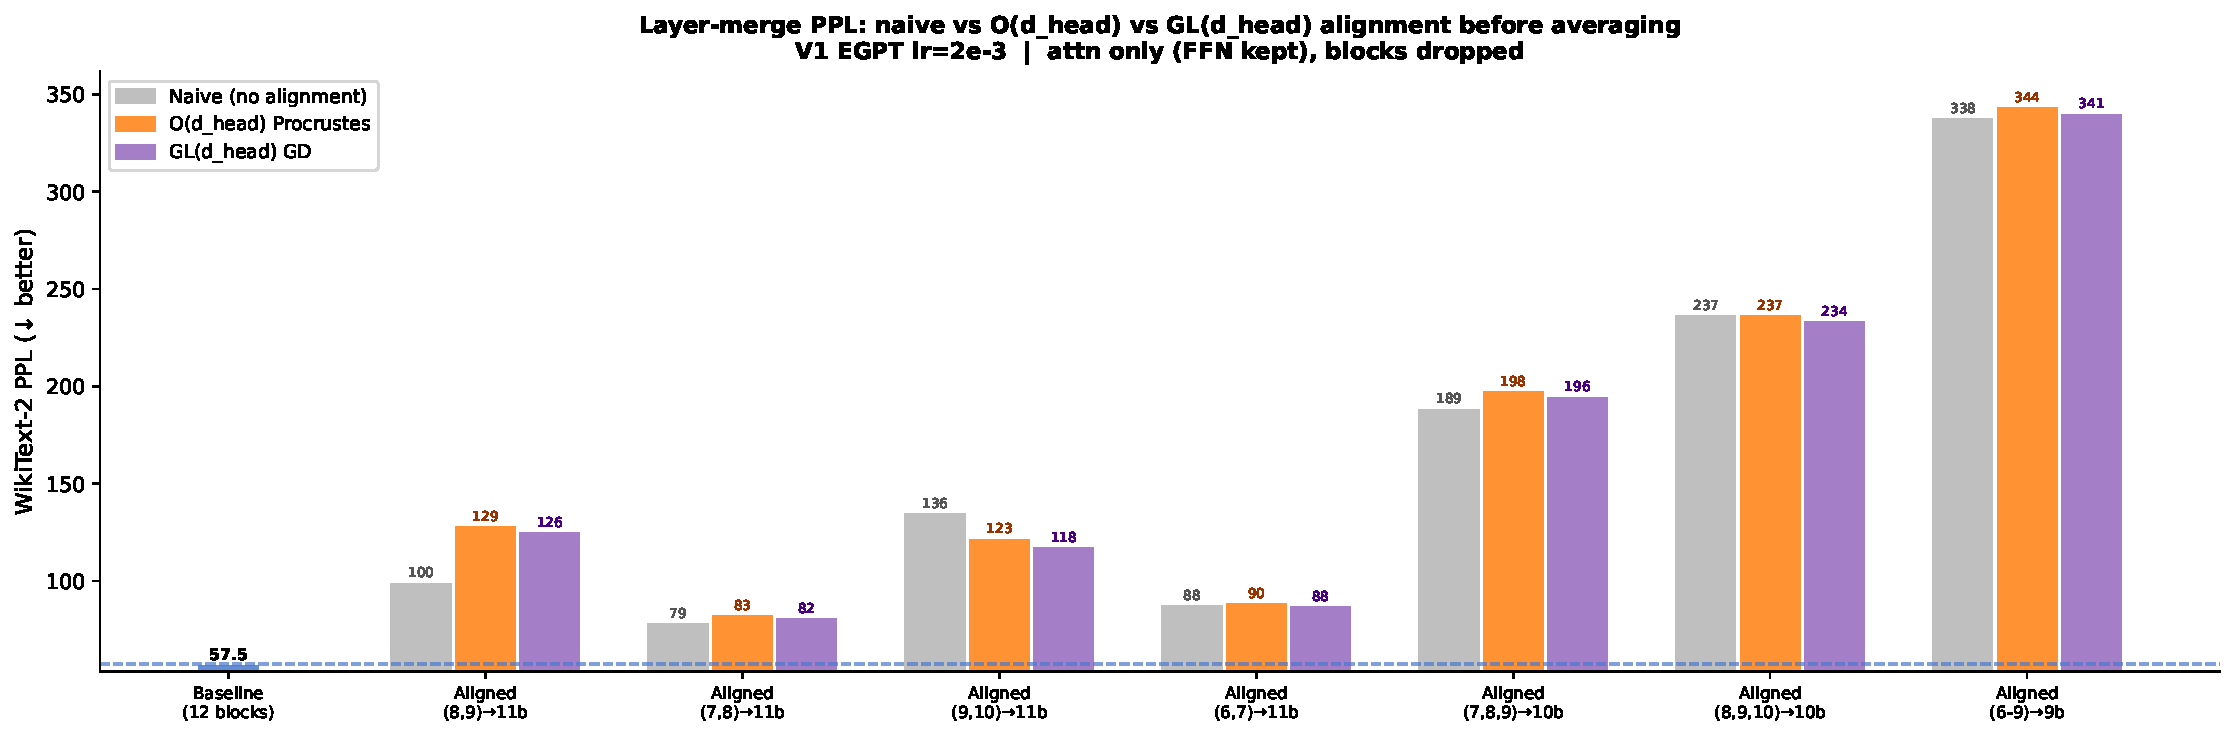
\includegraphics[width=\textwidth]{../results/multi-block-ablation/plots/layer_merge_aligned_ppl.pdf}
  \caption{Layer-merge PPL: naive (grey), O($d_h$) Procrustes (orange), GL($d_h$) GD (purple).
    Neither alignment strategy consistently reduces PPL degradation.
    The high output-space cosine similarity between adjacent EGPT layers
    is not explained by weight-space symmetries.}
  \label{fig:layer_merge_aligned_ppl}
\end{figure}

\paragraph{Interpretation.}
The high consecutive-layer attn\_out cosine similarity in EGPT (up to 0.53 for layers 8--9)
is a property of the \emph{function} computed, not of the \emph{weights} themselves.
Adjacent layers produce directionally similar attention outputs because EGPT's subtractive
update keeps the residual stream $h$ close to a shared attractor, so the attention modules
see similar inputs and compute similar directions --- not because the weight matrices are
structurally related.
Even the full GL($d_h$) symmetry group (scaling and shear, not just rotations) fails to
explain the similarity, ruling out zero-shot weight merging as a compression strategy.
Fine-tuning after merge, or block-drop (keeping one block intact),
remain viable alternatives and are left for future work.

%% ============================================================
\section{Learning Rate and Stability}
%% ============================================================

Training curves (WandB project \texttt{energy-inference-large}) reveal:
\begin{itemize}
  \item The GPT baseline (V0) at 3e-4 reaches lower loss at step 8k than V1 at step 20k,
    confirming EGPT's lower sample efficiency.
  \item V4 (shared backbone, wide heads) achieves the lowest EGPT training loss but is
    the slowest to train ($\sim$6k steps in 2 hours vs.\ V2's $\sim$25k steps/2hr on
    the same hardware).
  \item V4 at lr=2e-3 shows noticeably spikier loss curves than lr=3e-4, suggesting the
    shared-backbone architecture may be less stable at high learning rates.
  \item V1 at lr=2e-3 shows clean convergence and substantial benchmark gains,
    making it the recommended starting point for 400M-scale exploration.
\end{itemize}

\paragraph{muP scaling to 400M.}
Under maximal-update parametrisation, $\text{LR} \propto 1/d$.  Scaling from the
160M sweet-spot ($d=768$, LR$\sim$2e-3) to $d=1024$:
\[
  \text{LR}_{400M} \approx 2\text{e-3} \times \frac{768}{1024} \approx 1.5\text{e-3}.
\]
We use a conservative LR$=7\text{e-4}$ for the 400M run to avoid instability.

%% ============================================================
\section{Conclusions}
%% ============================================================

\begin{enumerate}
  \item \textbf{EGPT is substantially less compute-efficient than GPT.}
    A 400M EGPT model uses 4.4$\times$ more FLOPs per token than a 162M GPT and achieves
    only comparable benchmark performance.  At 160M iso-param scale, GPT leads on perplexity
    by 24\% (38.3 vs.\ 47.7 for the best EGPT variant).  The zero-shot gap is smaller ---
    the best 160M EGPT nearly ties GPT --- but this does not compensate for the perplexity
    and compute gaps.  An iso-compute 400M GPT baseline (not run here) would be expected to
    substantially outperform V1 400M EGPT.
  \item \textbf{The training loss tracking result is informative but not encouraging.}
    The 400M EGPT loss curve tracking the 162M GPT loss curve confirms that EGPT's effective
    compute utilisation is roughly $1/4$ of GPT's, not that the two models are equivalent.
  \item \textbf{Balanced curl--gradient structure is universal.}
    All trained projection matrices show $\|A\|_F / \|S\|_F \approx 1$, confirming that
    the EGPT update rule requires both conservative and dissipative dynamics, not just
    gradient descent.
  \item \textbf{Shared backbone is parameter-efficient.}
    V3 with one shared block iterated 12$\times$ matches V1 (12 distinct blocks $\times$ 1)
    on perplexity despite having far fewer unique parameters.
  \item \textbf{Mixed-head architectures do not improve over pure GPT.}
    Mixing energy (V=K) and GPT (V=W$_V$x) heads in the same block (V10/V11) matches
    pure GPT at iso-param scale but does not exceed it.  The V=K constraint is
    a structural bottleneck for perplexity regardless of the fraction of energy heads.
  \item \textbf{V9 GPT 354M closes the compute gap.}
    A 354M standard GPT trained on 7.86B tokens achieves 49.6\% avg accuracy and 29.84
    PPL, outperforming V1 400M EGPT (48.5\%, 38.6 PPL) with the same parameter count.
    The iso-compute comparison now strongly favours standard transformers.
  \item \textbf{Next steps}: the key open question is whether EGPT offers any advantage
    GPT cannot replicate with the same compute --- e.g., test-time scaling via extra
    recurrence steps, or stronger reasoning from RL-steered iterative refinement.
    Until that is demonstrated, the compute efficiency gap is the dominant result.
\end{enumerate}

%% ============================================================
\appendix
\section{Additional Benchmark Figures}
\label{app:benchmarks}
%% ============================================================

\begin{figure}[h]
  \centering
  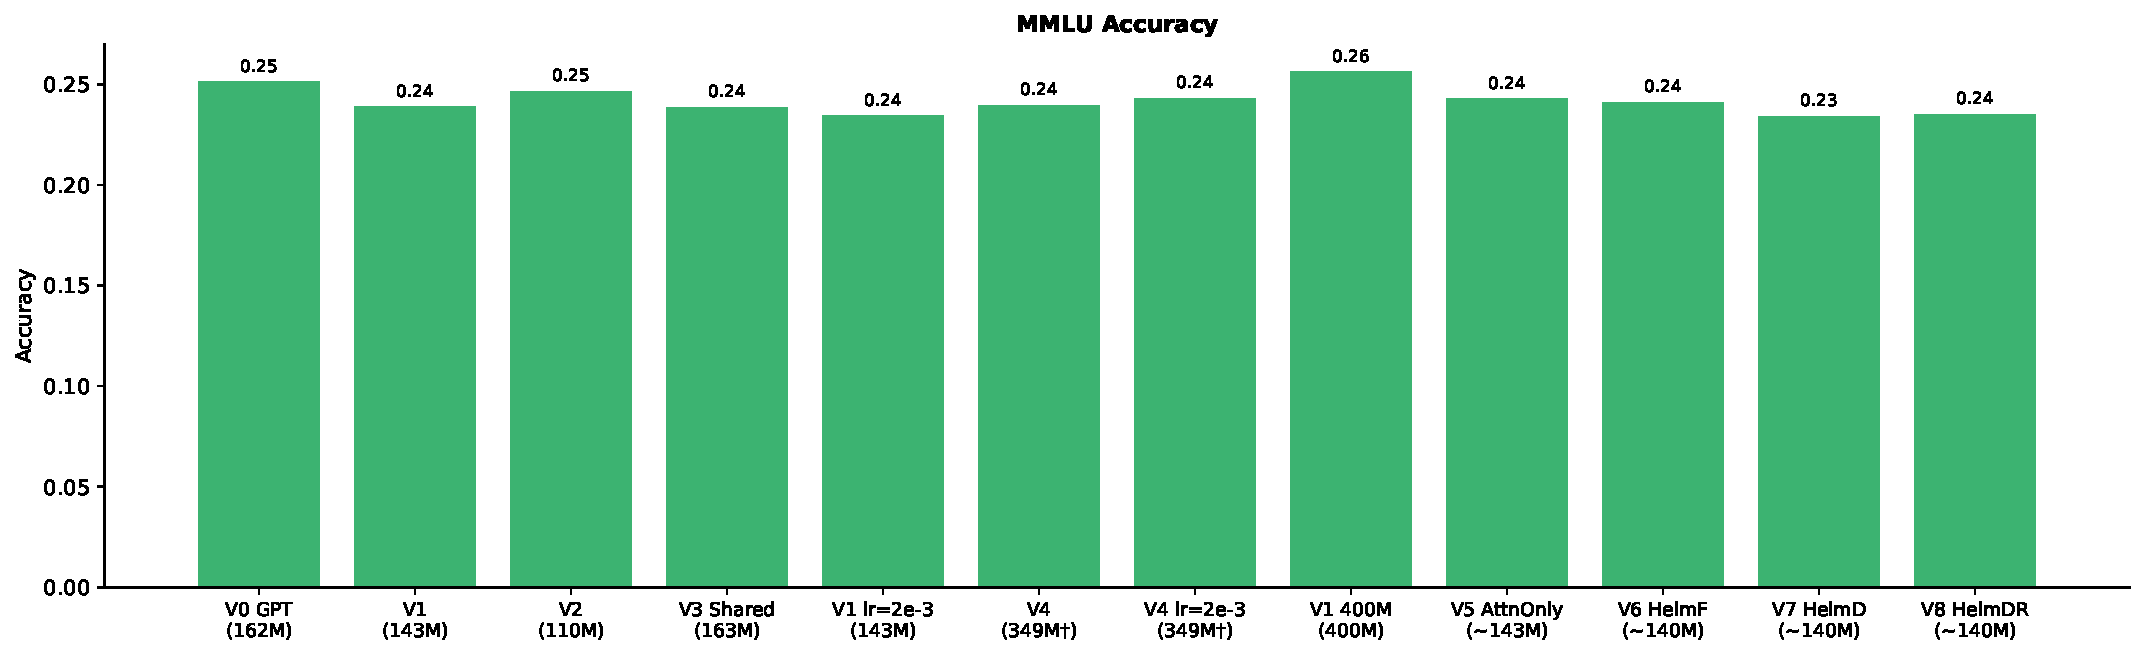
\includegraphics[width=0.6\textwidth]{../results/multi-block-ablation/plots/mmlu_acc.pdf}
  \caption{MMLU accuracy across all model variants.  All models perform near the
    random-chance baseline (0.25) at this scale; V1 400M (0.257) marginally leads
    V0 GPT (0.252).  MMLU requires factual knowledge that is unlikely to be acquired
    in 7.86B tokens.}
  \label{fig:mmlu}
\end{figure}

\begin{figure}[h]
  \centering
  \begin{subfigure}[b]{0.48\textwidth}
    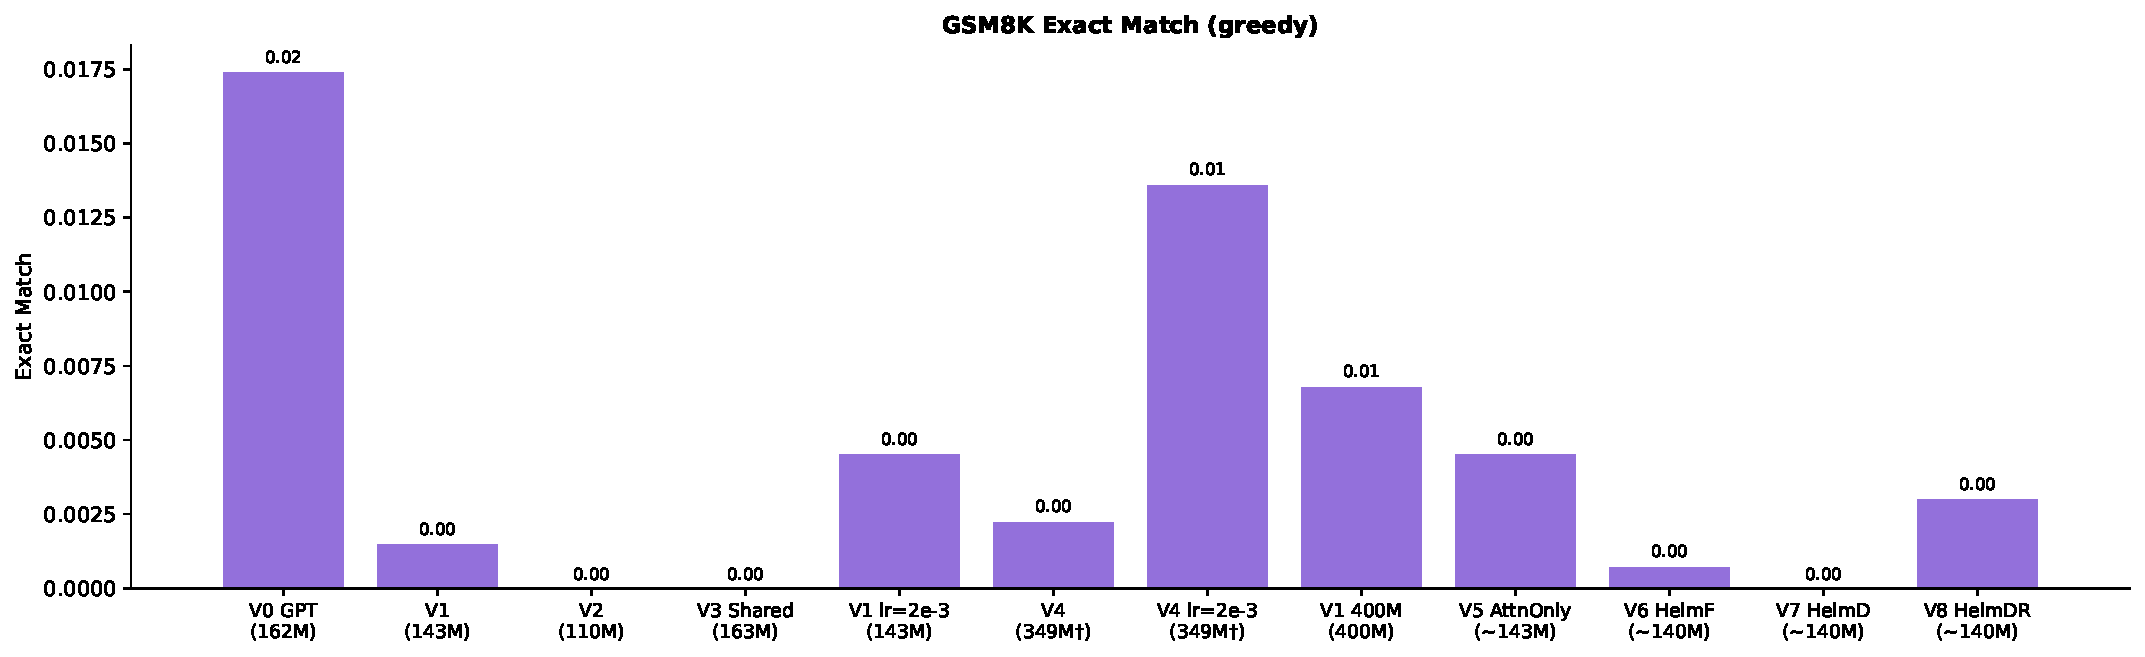
\includegraphics[width=\textwidth]{../results/multi-block-ablation/plots/gsm8k_acc.pdf}
    \caption{GSM8K greedy exact match.}
    \label{fig:gsm8k}
  \end{subfigure}
  \hfill
  \begin{subfigure}[b]{0.48\textwidth}
    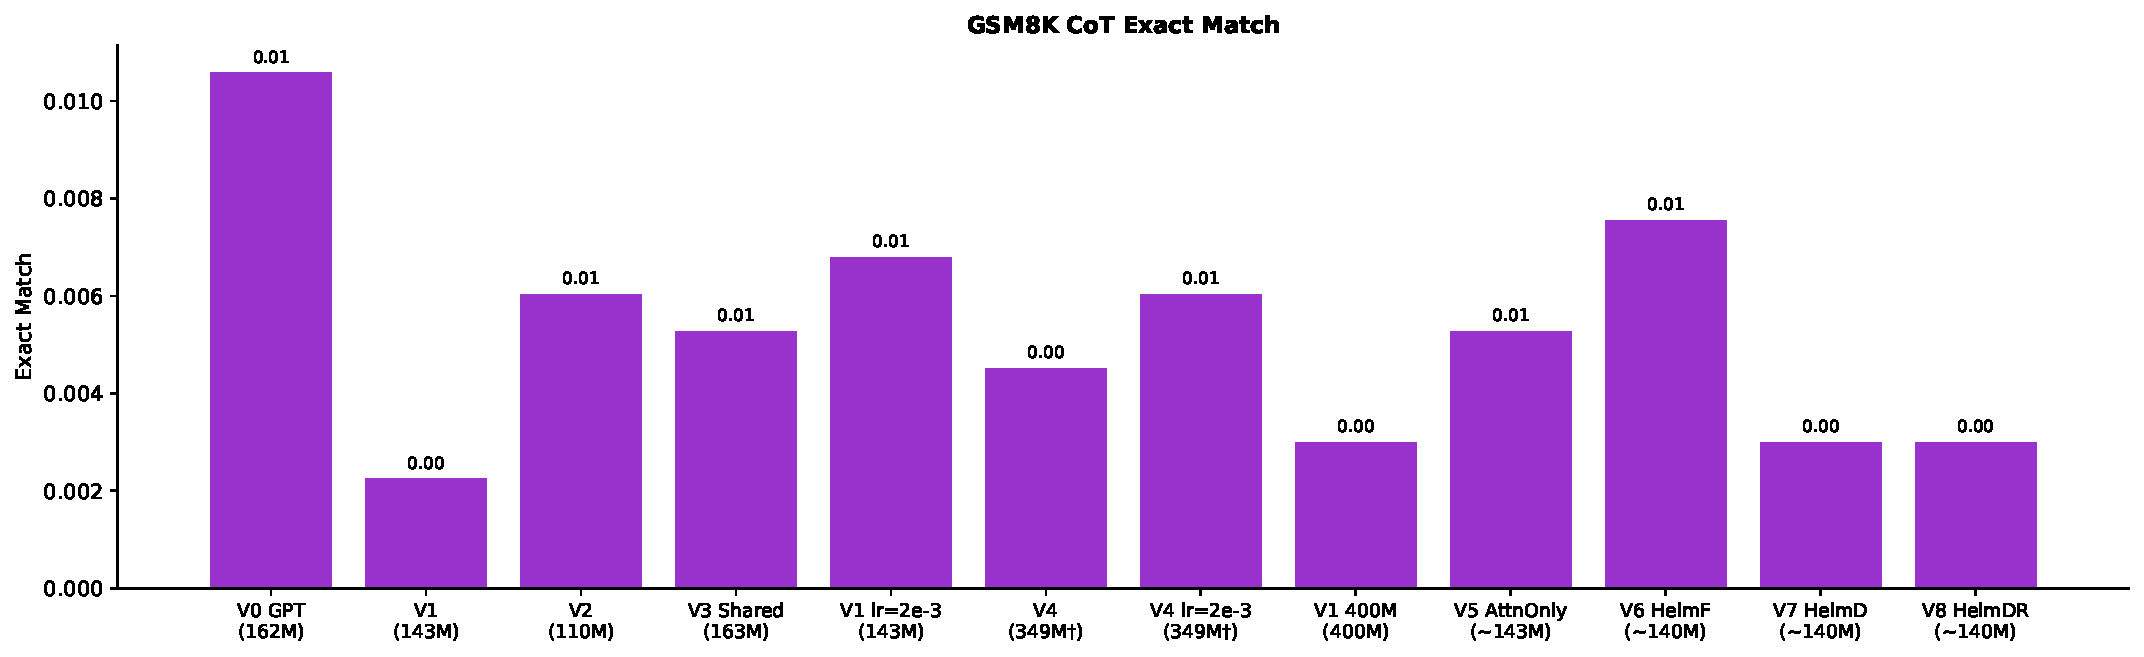
\includegraphics[width=\textwidth]{../results/multi-block-ablation/plots/gsm8k_cot_acc.pdf}
    \caption{GSM8K chain-of-thought exact match.}
    \label{fig:gsm8k_cot}
  \end{subfigure}
  \caption{GSM8K mathematical reasoning benchmarks.  All models score near zero at
    this scale.  V0 GPT leads on both greedy (0.017) and CoT (0.011).  Chain-of-thought
    prompting provides no benefit at 160M scale --- V4 lr=2e-3 is the only EGPT variant
    with non-trivial greedy performance (0.014).}
  \label{fig:gsm8k_combined}
\end{figure}

%% ============================================================
\section{Helmholtz Decomposition and Attention-Only Ablation (V5--V8)}
\label{app:helmholtz}
%% ============================================================

Variants V5--V8 test whether specific structural choices in V1's energy blocks are
necessary for performance:

\begin{itemize}
  \item \textbf{V5 (AttnOnly, 143M):} Energy attention with $V{=}K$ but \emph{no}
    projection MLP (\texttt{proj\_mlp} removed; 7.08M fewer parameters than V1).
    All 12 blocks are otherwise identical to V1.
  \item \textbf{V6 (HelmF, 140M):} Helmholtz-factored projections --- the projection
    matrix is explicitly split into symmetric (gradient) and anti-symmetric (curl)
    components with separate learned weights.
  \item \textbf{V7 (HelmD, 140M):} Dual Helmholtz --- attention uses the gradient
    component, FFN uses the curl component.
  \item \textbf{V8 (HelmDR, 140M):} Reversed dual Helmholtz --- attention uses curl,
    FFN uses gradient.
\end{itemize}

\begin{table}[h]
\centering
\caption{V5--V8 ablation results at 30k steps (7.86B tokens), 160M scale.
  ``Avg'' = mean over 9 zero-shot tasks. V0 GPT and V1 EGPT repeated for reference.
  WikiText PPL lower is better; zero-shot accuracy higher is better.}
\label{tab:v5_v8}
\resizebox{\textwidth}{!}{%
\begin{tabular}{lcccccccccccc}
\toprule
\textbf{Model} & \textbf{PPL}$\downarrow$ & \textbf{Avg}$\uparrow$
  & \textbf{ARC-c} & \textbf{ARC-e} & \textbf{Hella} & \textbf{Wino}
  & \textbf{BoolQ} & \textbf{PIQA} & \textbf{COPA} & \textbf{OBQA} & \textbf{SciQ} \\
\midrule
V0 GPT (162M)     & \textbf{38.3} & \textbf{0.491} & 0.245 & 0.459 & \textbf{0.330} & \textbf{0.517} & 0.566 & \textbf{0.632} & 0.590 & \textbf{0.296} & \textbf{0.781} \\
V1 EGPT (143M)    & 47.7 & 0.490 & 0.236 & 0.446 & 0.308 & 0.507 & \textbf{0.611} & 0.622 & \textbf{0.640} & 0.292 & 0.752 \\
\midrule
V5 AttnOnly (143M) & 48.6 & 0.483 & 0.239 & 0.448 & 0.306 & 0.514 & 0.572 & 0.628 & 0.620 & 0.286 & 0.737 \\
V6 HelmF (140M)   & 82.1 & 0.435 & 0.234 & 0.384 & 0.277 & 0.507 & 0.500 & 0.589 & 0.550 & 0.258 & 0.615 \\
V7 HelmD (140M)   & 63.4 & 0.451 & 0.221 & 0.413 & 0.287 & 0.507 & 0.472 & 0.608 & 0.610 & 0.270 & 0.667 \\
V8 HelmDR (140M)  & 65.2 & 0.457 & 0.232 & 0.423 & 0.286 & 0.503 & 0.539 & 0.602 & 0.570 & 0.272 & 0.689 \\
\bottomrule
\end{tabular}}
\end{table}

\paragraph{Key findings.}
\begin{enumerate}
  \item \textbf{V5 is close to V1 but measurably worse.}
    Removing the projection MLP (saving 7.08M parameters) costs $-0.7$ pp on average
    zero-shot accuracy (48.3\% vs.\ 49.0\%).  The BoolQ/COPA advantage over GPT is
    partially preserved (+0.6/+3.0 pp over V0), but reduced compared to V1
    (+4.5/+5.0 pp).  This confirms that the \texttt{proj\_mlp} contributes meaningfully,
    but the energy attention mechanism alone is responsible for most of the
    BoolQ/COPA effect.

  \item \textbf{Helmholtz variants (V6--V8) are significantly worse.}
    Explicitly enforcing the curl--gradient split via architectural decomposition
    degrades both perplexity (63--82 vs.\ 48 for V1) and zero-shot accuracy
    (43.5--45.7\% vs.\ 49.0\%).  This is counterintuitive given the curl--gradient
    analysis (Section~\ref{sec:curl_grad}) showing that trained V1 projections already
    exhibit balanced $\|A\|/\|S\|$ ratios --- the \emph{emergent} balance is
    beneficial, but \emph{forcing} it at initialisation and constraining the
    parameterisation hurts training dynamics.

  \item \textbf{V7 vs.\ V8: component assignment matters.}
    Assigning the gradient component to attention and curl to FFN (V7, 45.1\%)
    versus the reverse (V8, 45.7\%) makes little difference.  Both are far below
    the unconstrained V1 baseline, confirming the Helmholtz decomposition approach
    is architecturally suboptimal regardless of assignment.
\end{enumerate}

\begin{figure}[h]
  \centering
  \begin{subfigure}[b]{0.48\textwidth}
    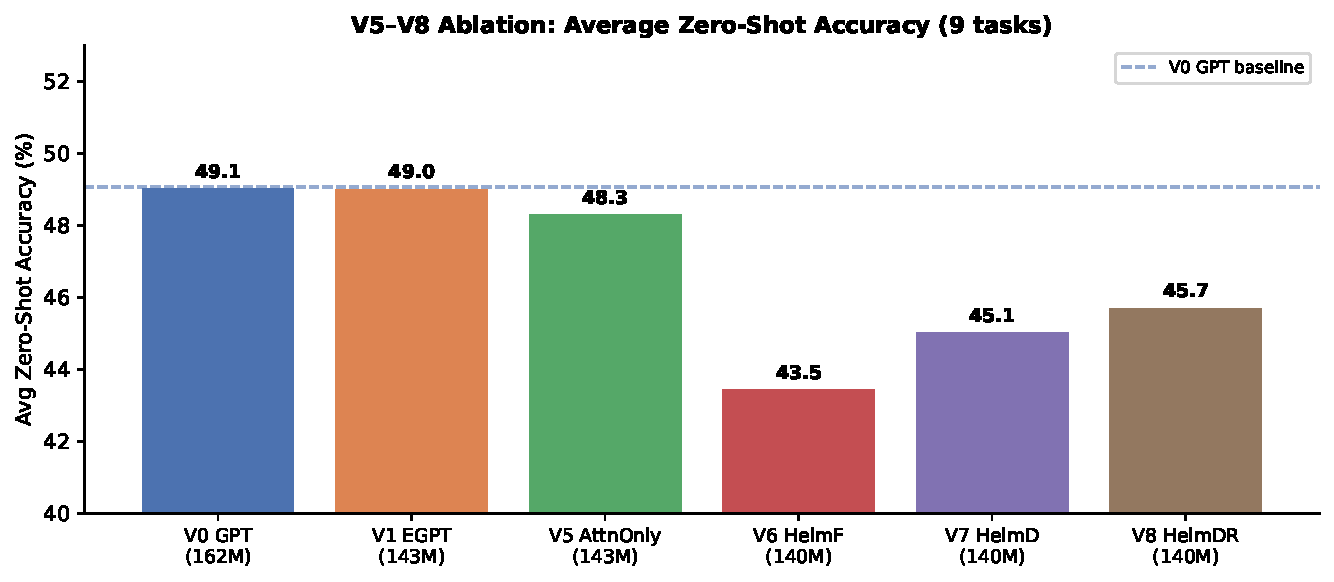
\includegraphics[width=\textwidth]{../results/multi-block-ablation/plots/v5_v8_avg_acc.pdf}
    \caption{Average zero-shot accuracy.  V5 stays close to V1; Helmholtz variants
      (V6--V8) drop 4--6 pp.}
    \label{fig:v5_v8_avg}
  \end{subfigure}
  \hfill
  \begin{subfigure}[b]{0.48\textwidth}
    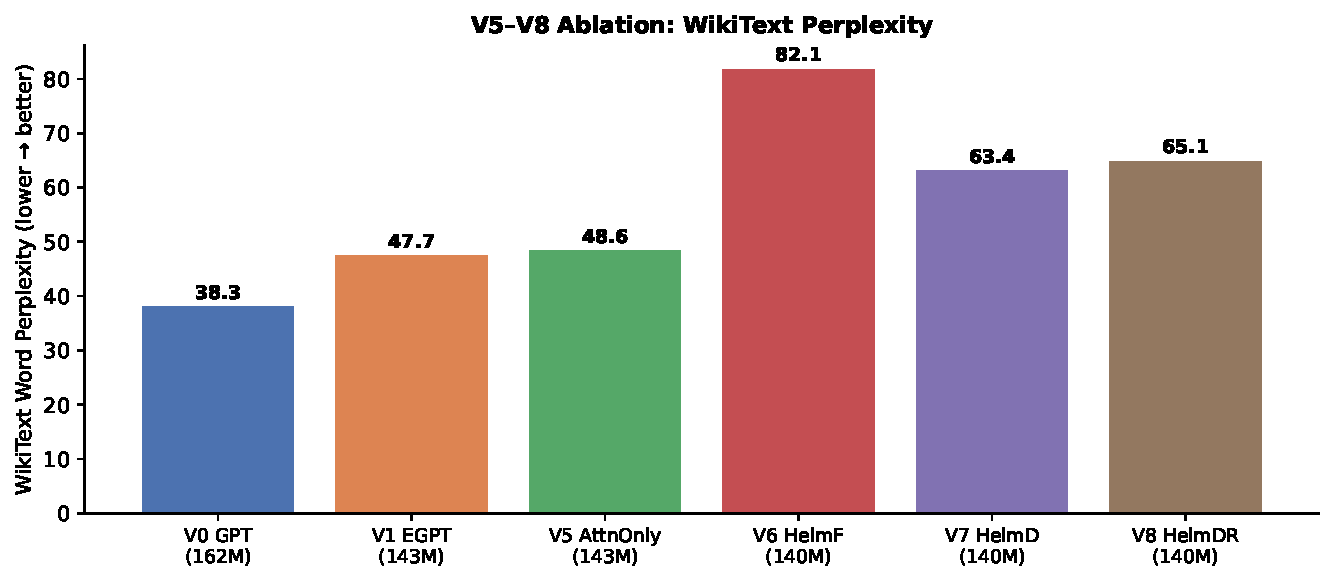
\includegraphics[width=\textwidth]{../results/multi-block-ablation/plots/v5_v8_wikitext_ppl.pdf}
    \caption{WikiText perplexity.  V6 (HelmF) spikes to 82.1; V7/V8 at 63--65 vs.\
      V1's 47.7.}
    \label{fig:v5_v8_ppl}
  \end{subfigure}
  \caption{V5--V8 ablation summary.  Dashed line = V0 GPT baseline (49.1\%).}
  \label{fig:v5_v8_summary}
\end{figure}

\begin{figure}[h]
  \centering
  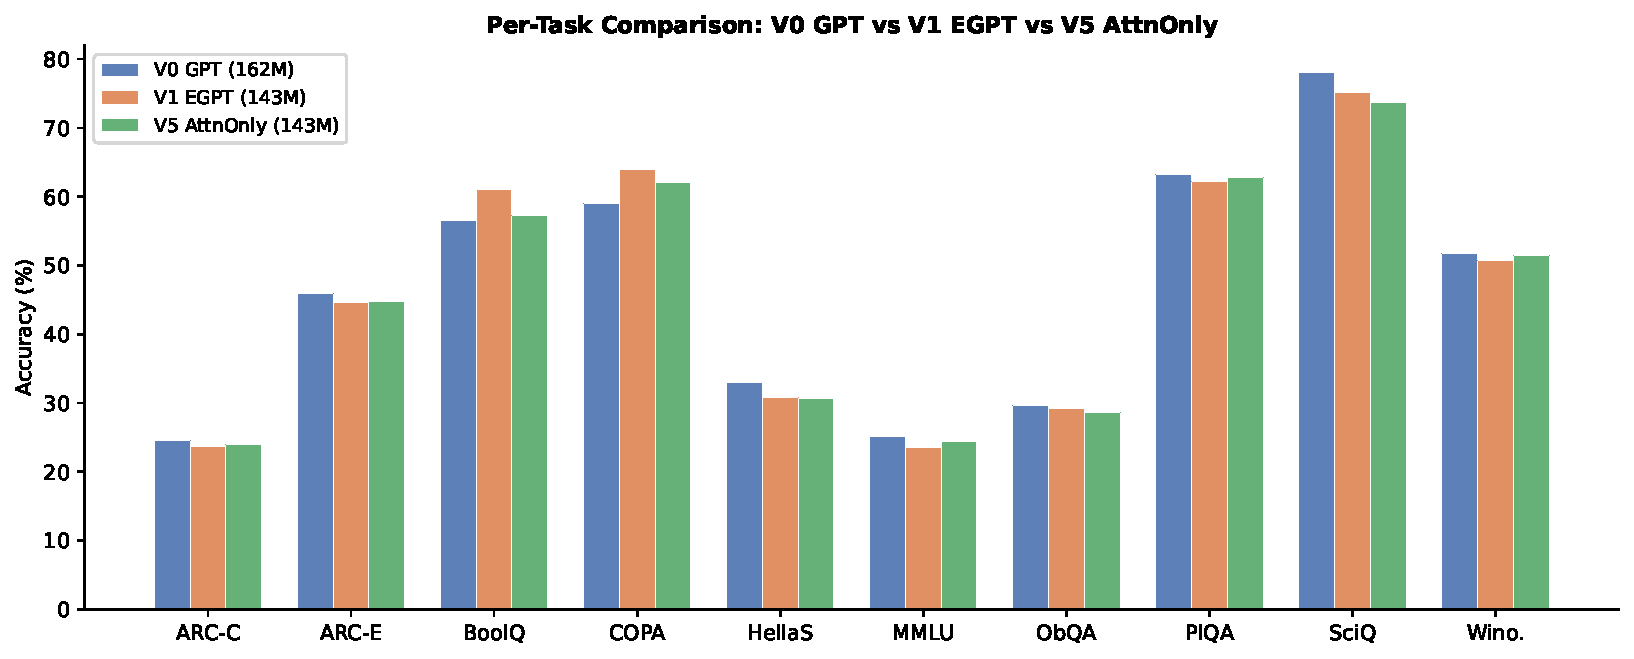
\includegraphics[width=\textwidth]{../results/multi-block-ablation/plots/v5_per_task.pdf}
  \caption{Per-task comparison of V0 GPT, V1 EGPT, and V5 (attention-only energy).
    V5 retains the BoolQ/COPA advantage but narrows it relative to V1, and trails
    GPT on knowledge/continuation tasks (ARC-e, HellaSwag, SciQ) by similar margins.}
  \label{fig:v5_per_task}
\end{figure}

\begin{figure}[h]
  \centering
  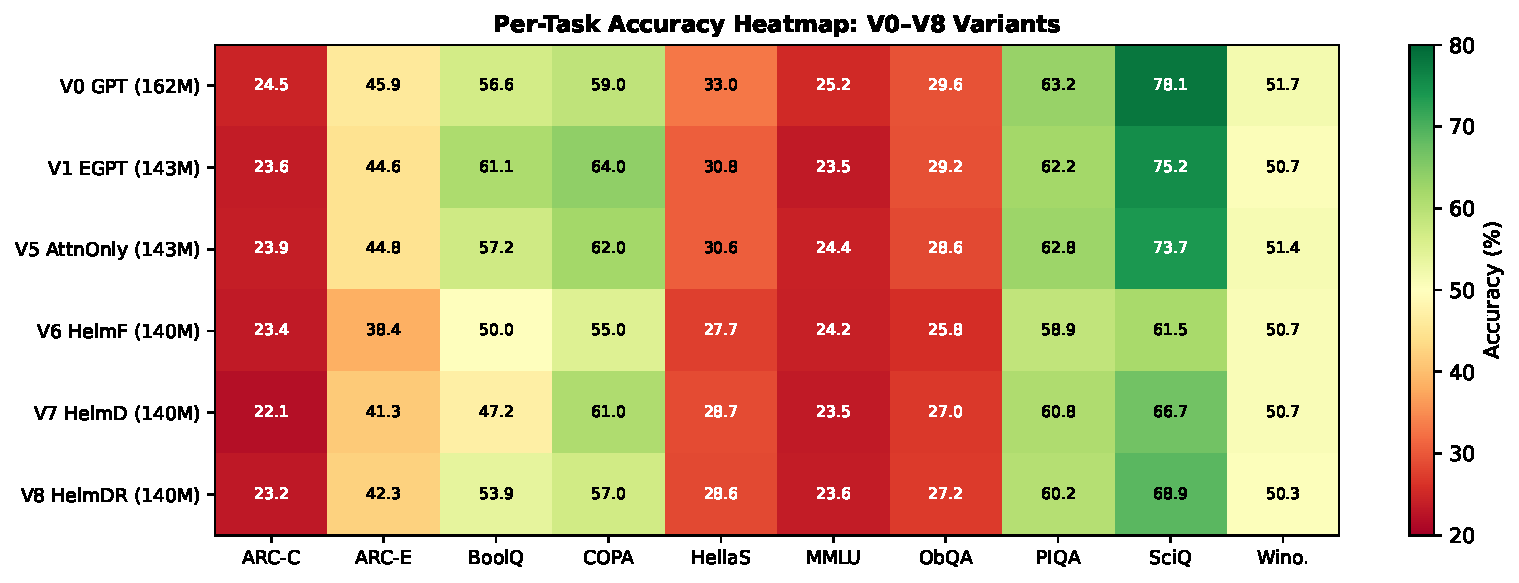
\includegraphics[width=\textwidth]{../results/multi-block-ablation/plots/v5_v8_heatmap.pdf}
  \caption{Per-task accuracy heatmap for V0--V8.  Colour encodes accuracy (green =
    high, red = low).  V6--V8 show broad degradation across all tasks.
    BoolQ column: V1 and V5 stand out as the brightest EGPT entries.}
  \label{fig:v5_v8_heatmap}
\end{figure}

%% ============================================================
\section{Mixed EGPT+GPT Heads (V10, V11): Iso-Family Comparison}
\label{app:mixed}
%% ============================================================

\paragraph{Motivation and design.}
The previous ablations test pure EGPT (V=K) and pure GPT (V=W$_V$x) architectures.
A natural middle ground is a \emph{mixed-head} model where a fraction of attention
heads use the energy constraint (V=K) and the remainder use a standard value projection.
We implement this as a single flash-attention kernel over all heads with a shared output
projection $W_O$: no separate forward pass, no additional modules.

\paragraph{Architecture details.}

\begin{table}[h]
\centering
\caption{Architecture and compute for the iso-family comparison.
  FLOPs/token = forward pass, $s{=}4096$, including attention kernel.
  Non-recurrent (12$\times$1) and recurrent (6$\times$2) families both apply
  12 block computations per token.}
\label{tab:mixed_arch}
\resizebox{\textwidth}{!}{%
\begin{tabular}{lrrrrrrr}
\toprule
\textbf{Model} & \textbf{Type} & \textbf{Layers} & \textbf{Iters} & \textbf{$d$} & \textbf{Int} & \textbf{Params} & \textbf{MFLOPs/tok} \\
\midrule
V0 GPT     & softmax attn     & 12 & 1 & 768 & 2048 & 162M & 321 \\
V1 EGPT    & energy (V=K)     & 12 & 1 & 768 & 2048 & 143M & 359 \\
V10 Mixed  & 6E+6G heads      & 12 & 1 & 768 & 1536 & 144M & 285 \\
\midrule
V2 EGPT    & energy (V=K)     &  6 & 2 & 768 & 2048 & 110M & 359 \\
V11 Mixed  & 6E+6G heads      &  6 & 2 & 768 & 2048 & 118M & 314 \\
V12 GPT    & softmax attn     &  6 & 2 & 768 & 2048 & 120M & 321 \\
\bottomrule
\end{tabular}}
\end{table}

\noindent\textit{Note:} V10 uses int$=1536$ to match V1's parameter count; V11 uses int$=2048$
matching V0/V2.  V1 and V2 EGPT have higher FLOPs/token than V0 GPT despite fewer parameters
because the energy MLP requires four matrix multiplications (W1$x$, W2$x$, gradient contractions)
vs.\ three for SwiGLU.

\paragraph{Results.}

\begin{table}[h]
\centering
\caption{Iso-family benchmark results.  All evals use \texttt{lm-evaluation-harness}.
  Arrows indicate improvements relative to same-family EGPT baseline.}
\label{tab:mixed_results}
\resizebox{\textwidth}{!}{%
\begin{tabular}{lrrrrrrr}
\toprule
\textbf{Metric} & \textbf{V0 GPT} & \textbf{V1 EGPT} & \textbf{V10 Mixed} & \textbf{V2 EGPT} & \textbf{V11 Mixed} & \textbf{V12 GPT} \\
 & 162M/321M$\dagger$ & 143M/359M & 144M/285M & 110M/359M & 118M/314M & 120M/321M \\
\midrule
Wikitext PPL $\downarrow$ & 38.31 & 47.66 & \textbf{36.99} & 63.32 & 40.67 & \textbf{39.98} \\
\textbf{Avg acc} $\uparrow$ & 47.2\% & 46.8\% & 47.2\% & 44.7\% & \textbf{47.3\%} & 47.0\% \\
GSM8K $\uparrow$       & \textbf{2.20\%} & 1.74\% & 1.52\% & 1.97\% & 1.36\% & 2.05\% \\
\midrule
ARC-Challenge & 24.5 & 23.6 & \textbf{25.5} & 22.5 & 24.5 & 24.0 \\
ARC-Easy      & 51.6 & 47.9 & 51.4 & 44.9 & 51.0 & \textbf{52.0} \\
BoolQ         & 56.6 & \textbf{61.1} & 56.5 & 61.0 & 58.6 & 56.7 \\
COPA          & 59.0 & \textbf{64.0} & 57.0 & 56.0 & 61.0 & 58.0 \\
HellaSwag     & 33.0 & 30.8 & \textbf{33.4} & 28.3 & 32.3 & 32.3 \\
OpenBookQA    & 29.6 & 29.2 & 27.4 & 28.2 & 29.4 & \textbf{30.8} \\
PIQA          & 63.2 & 62.2 & \textbf{65.4} & 61.4 & 63.4 & 63.1 \\
SciQ          & \textbf{78.1} & 75.2 & 76.9 & 69.3 & 75.7 & 77.7 \\
Winogrande    & 51.7 & 50.7 & \textbf{52.7} & 50.7 & 51.8 & 50.6 \\
MMLU          & 25.2 & 23.5 & \textbf{25.7} & 24.7 & 24.9 & 24.7 \\
\bottomrule
\end{tabular}}
\end{table}
\noindent$\dagger$ Params/MFLOPs per token.

\begin{figure}[h]
  \centering
  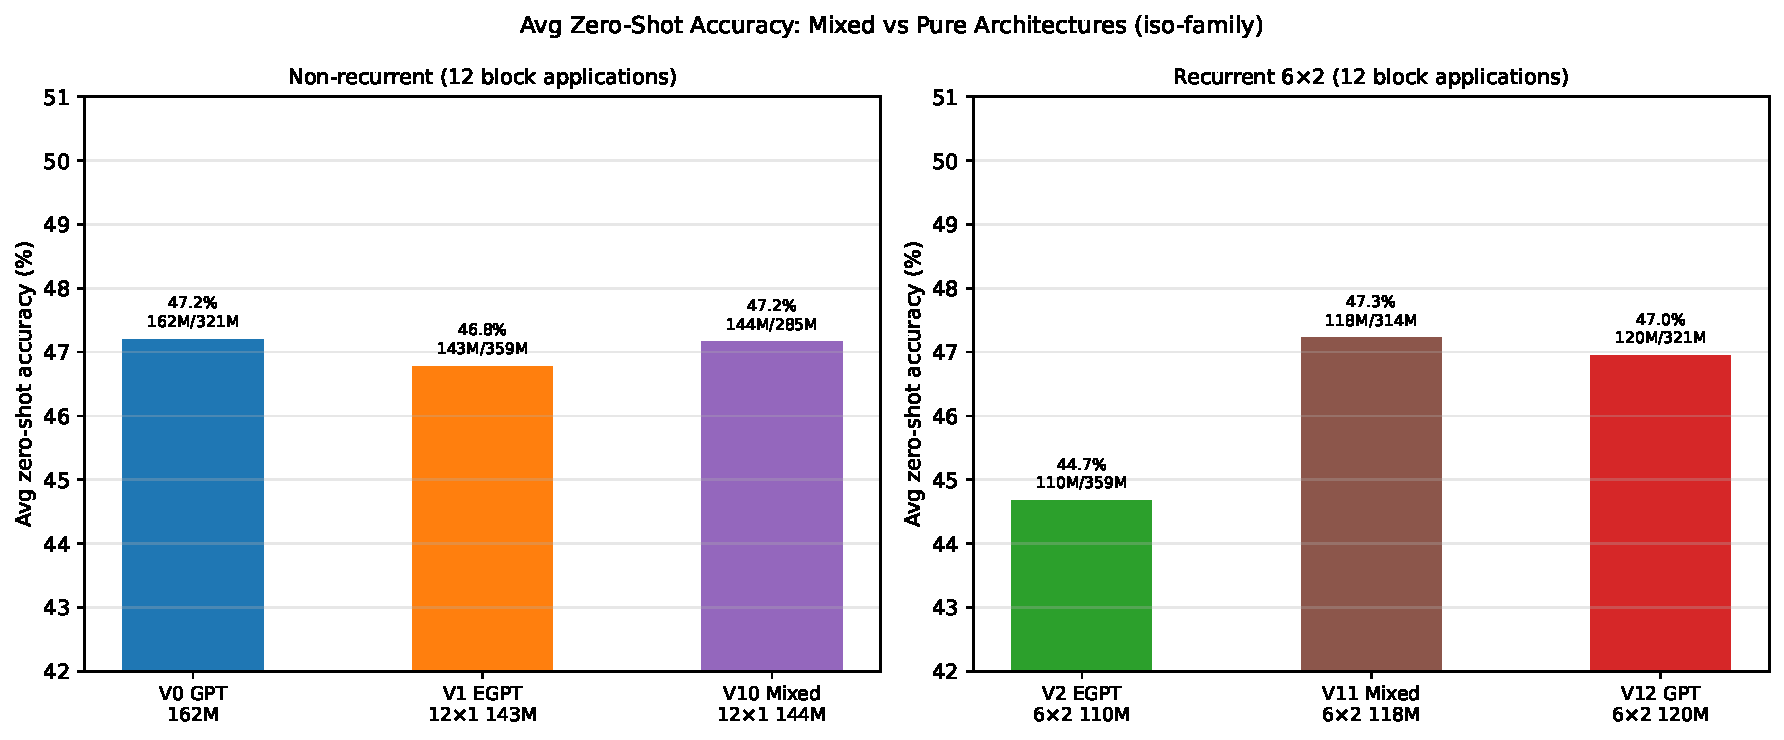
\includegraphics[width=\textwidth]{../results/multi-block-ablation/plots/mixed_iso_avg_acc.pdf}
  \caption{Average accuracy grouped by architecture family.
    Left: non-recurrent 12$\times$1; right: recurrent 6$\times$2.
    Bar labels show params\,/\,FLOPs per token.
    V10 matches V0 with 11\% fewer FLOPs; V11 beats V2 by $+2.6$pp with 13\% fewer FLOPs.}
  \label{fig:mixed_avg_acc}
\end{figure}

\begin{figure}[h]
  \centering
  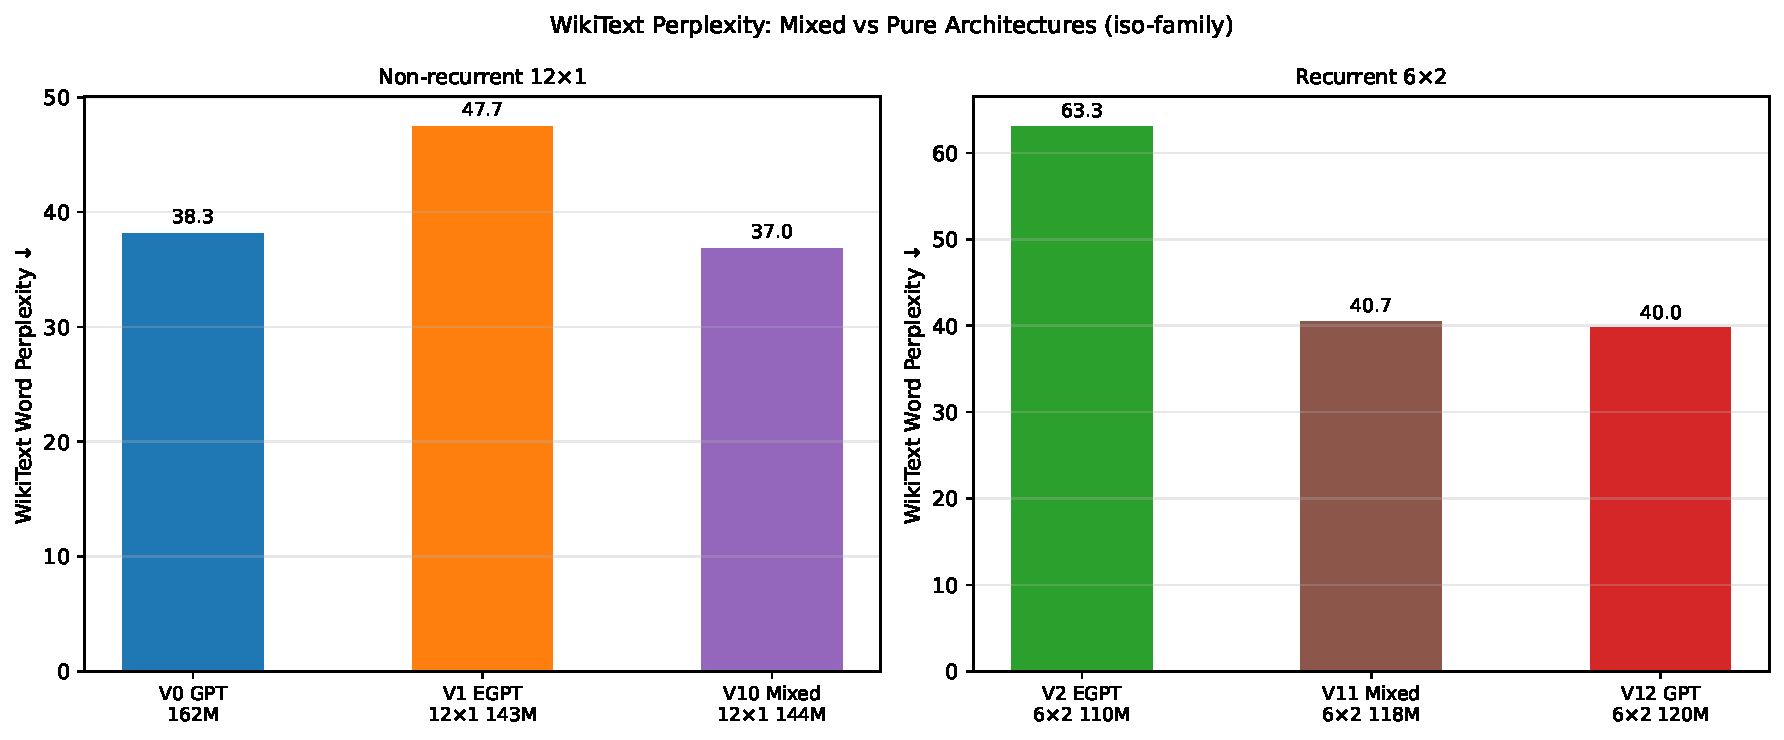
\includegraphics[width=\textwidth]{../results/multi-block-ablation/plots/mixed_iso_ppl.pdf}
  \caption{WikiText perplexity by family.  Mixed models substantially improve EGPT PPL
    ($-10.7$ for V10 vs V1; $-22.6$ for V11 vs V2) without sacrificing accuracy.}
  \label{fig:mixed_ppl}
\end{figure}

\begin{figure}[h]
  \centering
  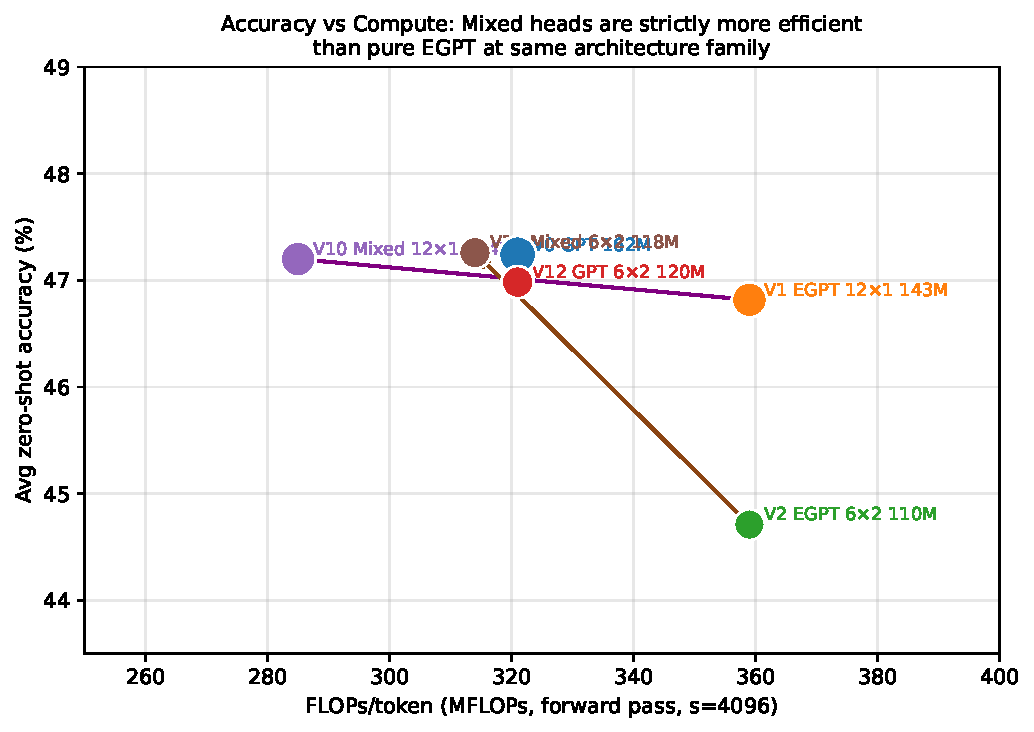
\includegraphics[width=0.65\textwidth]{../results/multi-block-ablation/plots/mixed_flops_vs_acc.pdf}
  \caption{Accuracy vs.\ FLOPs/token.  Arrows show the gain from replacing pure EGPT
    with mixed heads: both V10 (purple) and V11 (brown) move left (fewer FLOPs) and up
    (higher accuracy) relative to their EGPT counterparts.  V0 GPT remains the frontier
    for the 12$\times$1 family.}
  \label{fig:mixed_flops}
\end{figure}

\begin{figure}[h]
  \centering
  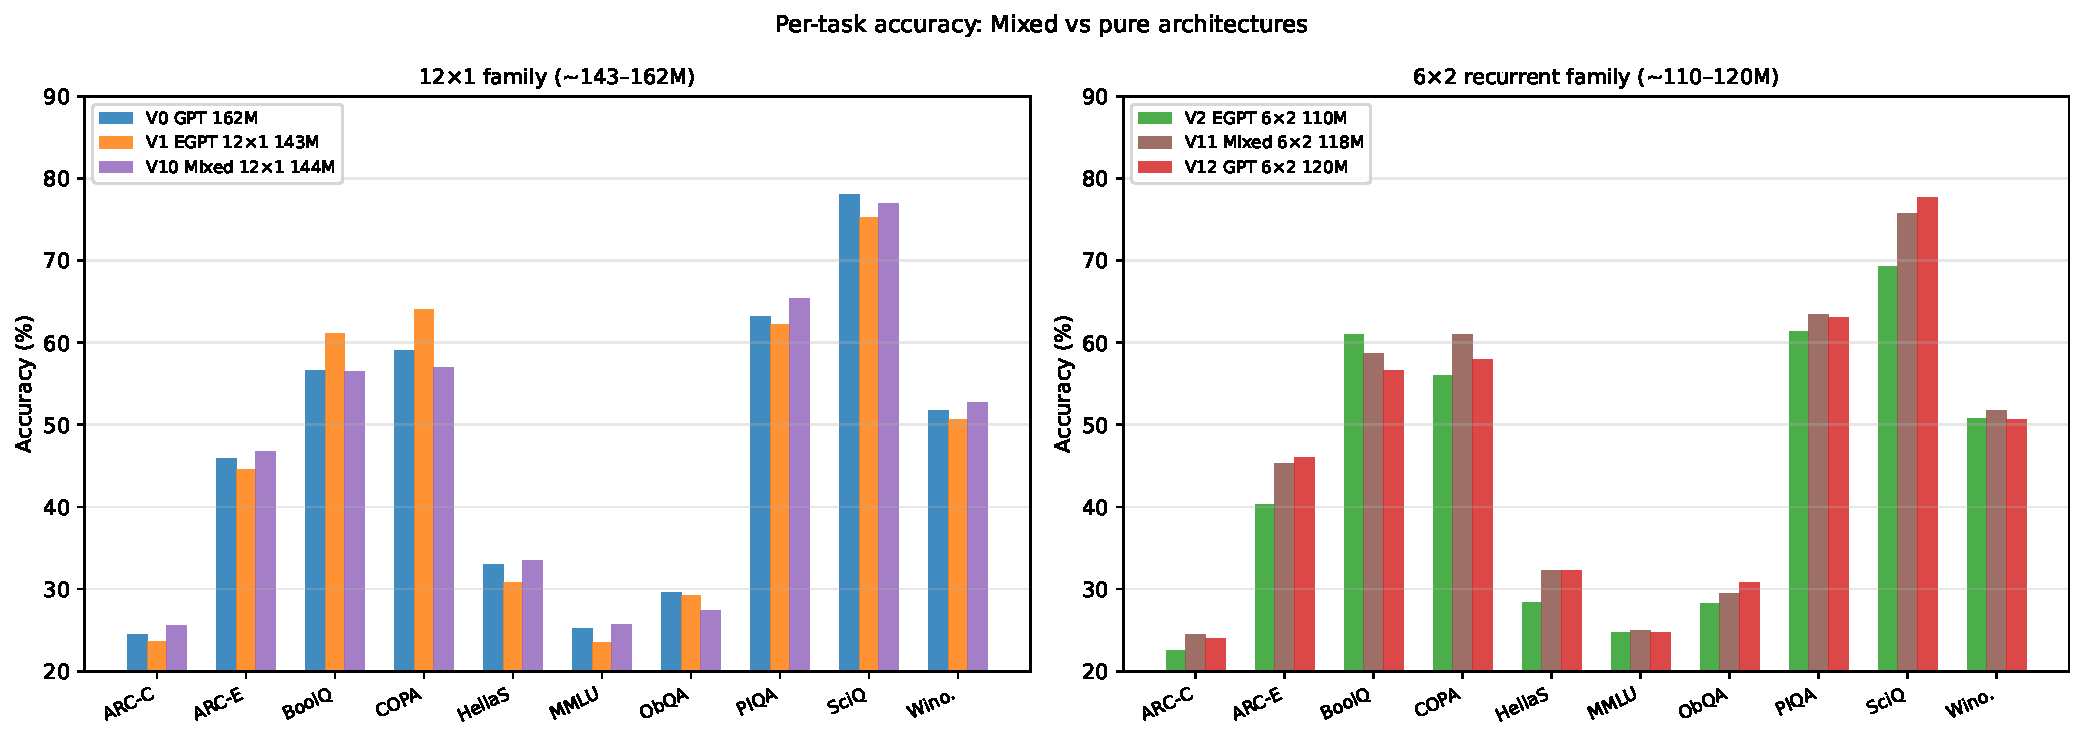
\includegraphics[width=\textwidth]{../results/multi-block-ablation/plots/mixed_per_task.pdf}
  \caption{Per-task accuracy for both iso-families.  Mixed models track V0 GPT closely
    on most tasks; V11 recovers the accuracy gap between V2 EGPT and V0 GPT on
    ARC-Easy, HellaSwag, PIQA, and SciQ.}
  \label{fig:mixed_per_task}
\end{figure}

\begin{figure}[h]
  \centering
  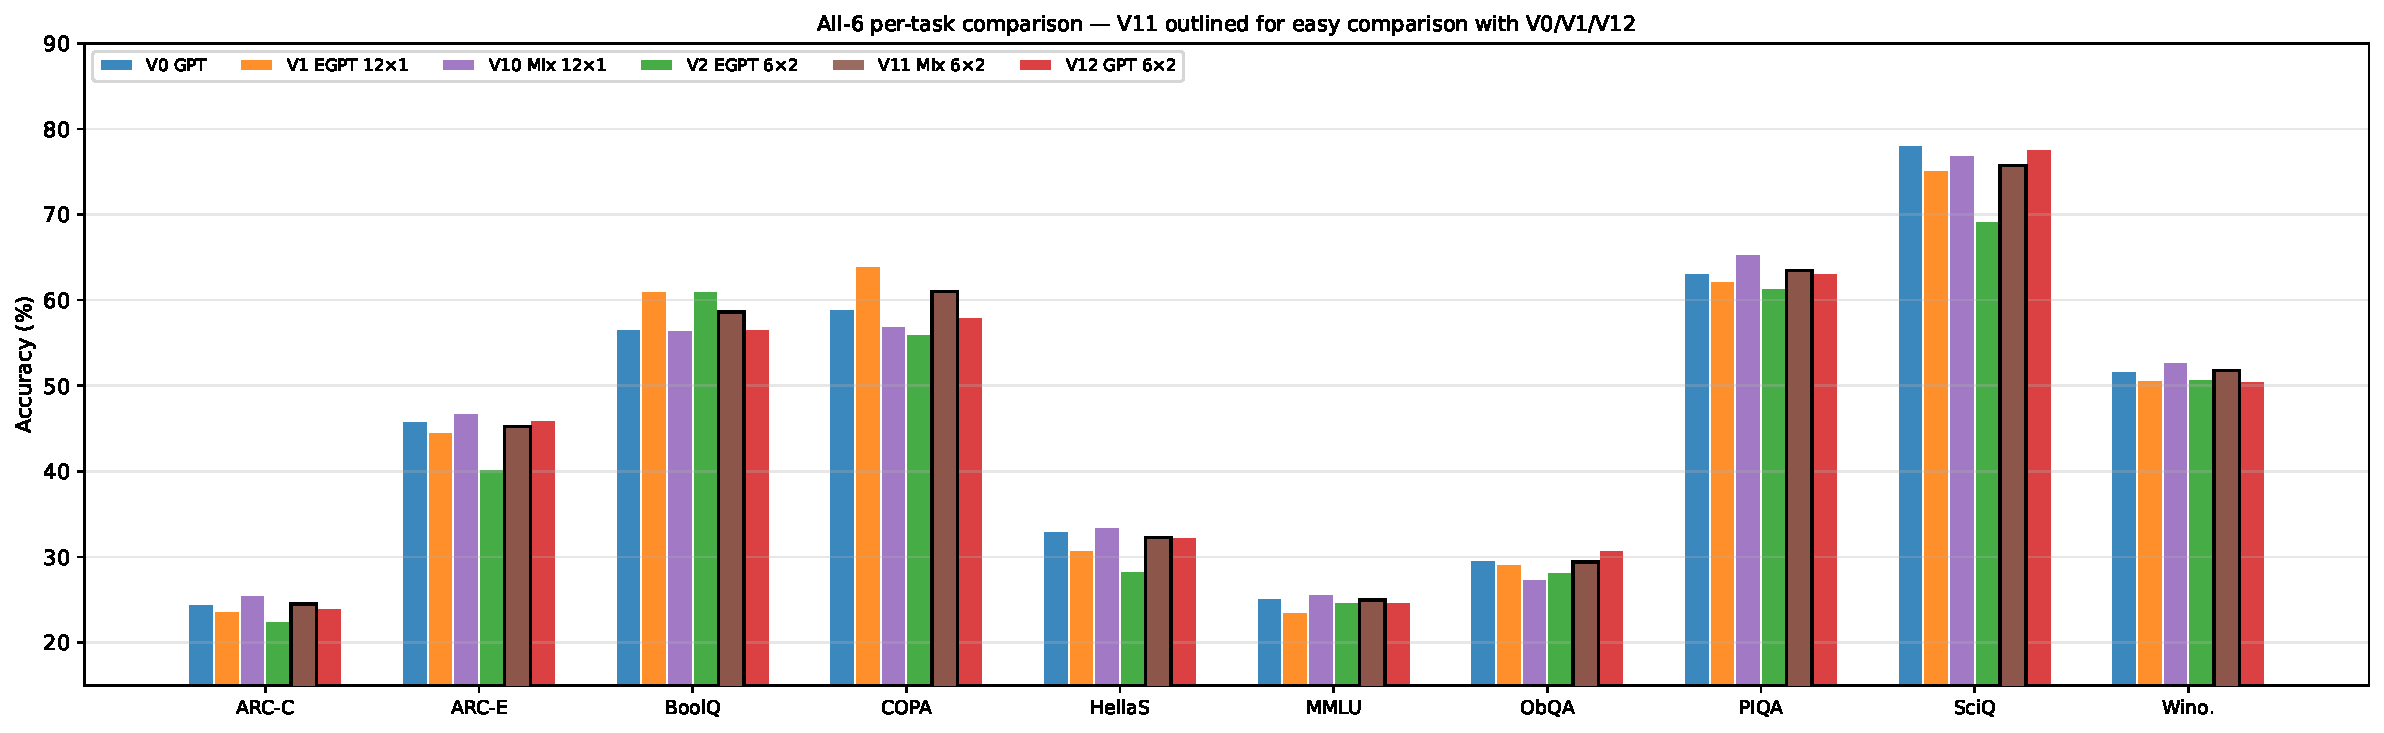
\includegraphics[width=\textwidth]{../results/multi-block-ablation/plots/mixed_all5_per_task.pdf}
  \caption{Per-task accuracy for all six iso-family models (V0 GPT, V1 EGPT 12$\times$1, V10 Mixed 12$\times$1,
    V2 EGPT 6$\times$2, V11 Mixed 6$\times$2, V12 GPT 6$\times$2).  V11 bars are outlined in black for easy
    direct comparison with the V0 GPT baseline and V1 EGPT.}
  \label{fig:mixed_all5_per_task}
\end{figure}

\begin{figure}[h]
  \centering
  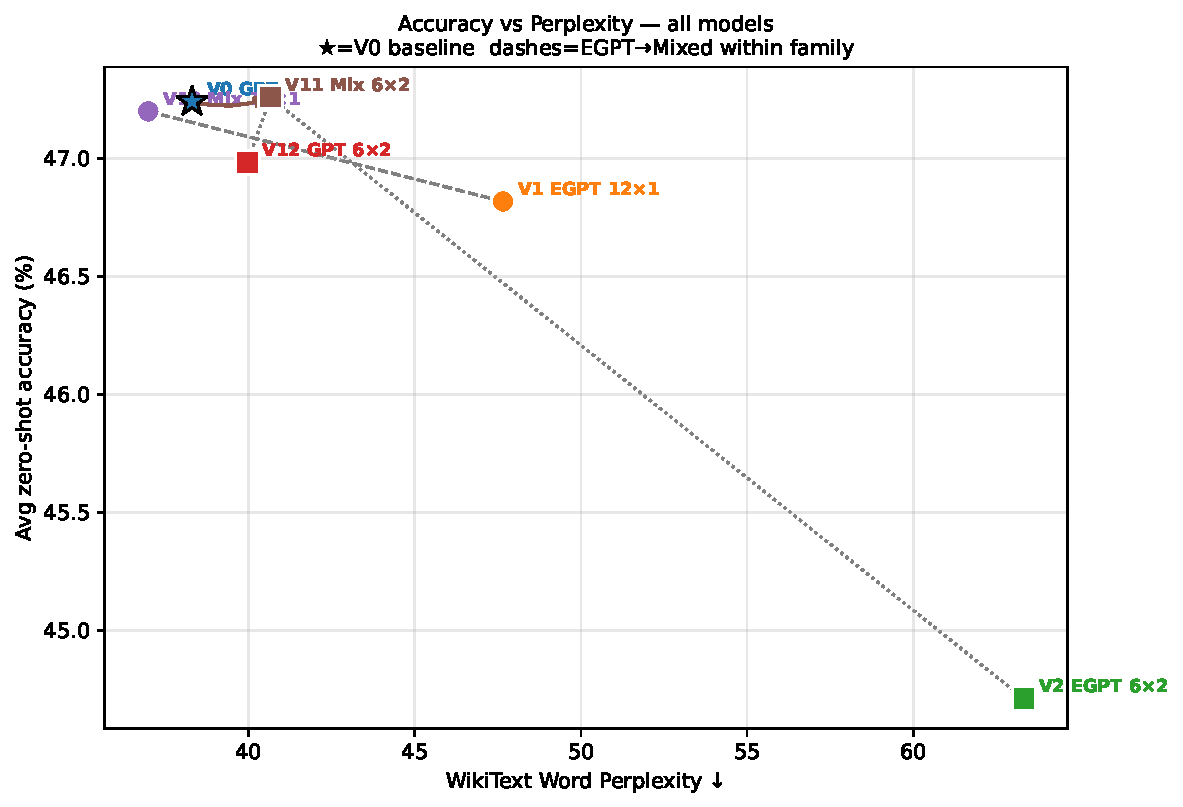
\includegraphics[width=0.75\textwidth]{../results/multi-block-ablation/plots/mixed_all5_ppl_vs_acc.pdf}
  \caption{Average zero-shot accuracy vs.\ WikiText word perplexity for all six models.
    Dashed lines connect models within each recurrence family.
    V11 matches V0 accuracy while reducing PPL, at lower parameter count;
    V12 (recurrent GPT) provides a strong non-energy 6$\times$2 baseline.  $\bigstar$\,=\,V0 GPT reference.}
  \label{fig:mixed_all5_ppl_vs_acc}
\end{figure}

\paragraph{Do mixed heads get the best of both worlds?}
\begin{enumerate}
  \item \textbf{Strictly better than pure EGPT in both families.}
    V10 improves over V1 EGPT on accuracy (+0.4pp), PPL ($-10.7$), and FLOPs ($-21\%$) simultaneously.
    V11 improves over V2 EGPT on accuracy (+2.6pp), PPL ($-22.6$), and FLOPs ($-13\%$).
    Replacing energy heads with GPT heads for half the heads is an unambiguous win over
    the fully-energy baseline.
  \item \textbf{Mixed matches but does not exceed V0 GPT on accuracy.}
    V10 ties V0 on average accuracy (47.2\%) with 12\% fewer parameters and 11\% fewer
    FLOPs, and achieves slightly better PPL (37.0 vs.\ 38.3).  On a strict per-FLOP basis,
    V10 is marginally more efficient than V0 at this scale.
    However, V0 GPT leads on GSM8K (2.20\% vs.\ 1.52\% for V10) and COPA.
  \item \textbf{No ``best of both worlds'' on GSM8K.}
    Both mixed models score below all pure baselines on GSM8K: V10 1.52\%, V11 1.36\%,
    vs.\ V0 2.20\%, V1 1.74\%, V2 1.97\%.
    The energy head V=K constraint appears to interfere with multi-step arithmetic
    reasoning regardless of the fraction of energy heads.
  \item \textbf{Recurrence does not help mixed heads (V11 vs.\ V10).}
    V11 (6$\times$2, 118M) achieves 47.3\% vs.\ V10's 47.2\% --- essentially the same.
    Iterating mixed-head blocks does not produce the structured refinement that
    motivates pure EGPT recurrence.
\end{enumerate}

\paragraph{GPT 400M iso-param baseline (V9).}
For completeness: V9 (standard GPT, 354M params, $d{=}1024$, 24 layers, lr$=1.5\!\times\!10^{-3}$)
achieves 49.6\% average accuracy and 29.84 PPL at 30k steps --- outperforming
V1 400M EGPT (48.5\%, 38.6 PPL) with identical parameter count.
This confirms that the compute efficiency gap between GPT and EGPT persists at 400M scale.

\subsection{Output-Rule Ablation: Energy Gradient and Energy Descent (V15, V16)}

The iso-family results (Section~\ref{sec:mixed}) showed that replacing half the energy
heads with standard GPT heads (V10) matches V0 GPT accuracy at fewer FLOPs, but does not
improve above the GPT baseline.  We next ask whether changing the \emph{output rule} of
the energy heads can close this gap.  Two variants are tested, both using the same
6E+6G head configuration as V10 and iso-param at 144M / 285 MFLOPs/tok:

\begin{itemize}
  \item \textbf{V15 EGrad}: Energy heads output the true energy gradient
    $W_Q^\top \sigma(QK^\top\!/\!\sqrt{d_h})\,K$ (where $\sigma$ is softmax)
    instead of $\sigma(\cdot)V$ with $V{=}K$.  GPT heads remain additive.
  \item \textbf{V16 EDesc}: The mixed-head output is used as a gradient direction:
    $h \leftarrow h - \mathrm{attn\_out}$,
    with no extra projection parameters (\texttt{energy\_proj\_type: identity}).
\end{itemize}

\begin{table}[h]
\centering
\caption{Output-rule ablation results (all 12$\times$1, $d{=}768$, 30k steps).
  V13/V14 eval pending.  \textbf{Bold} = best per metric.}
\label{tab:new_variants}
\resizebox{\textwidth}{!}{%
\begin{tabular}{lrrrrrrrrrrrrr}
\toprule
\textbf{Metric} & \textbf{V0 GPT} & \textbf{V1 EGPT} & \textbf{V10 Mix} & \textbf{V15 EGrad} & \textbf{V16 EDesc} \\
 & 162M/321M & 143M/359M & 144M/285M & 144M/285M & 144M/285M \\
\midrule
Wikitext PPL $\downarrow$ & 38.31 & 47.66 & 36.99 & \textbf{36.96} & 36.98 \\
\textbf{Avg acc} $\uparrow$ & 47.2\% & 46.8\% & 47.2\% & \textbf{47.9\%} & 47.4\% \\
GSM8K $\uparrow$       & 2.20\% & 1.74\% & 1.52\% & \textbf{2.58\%} & 2.20\% \\
\midrule
ARC-Challenge & 24.5 & 23.6 & \textbf{25.5} & 24.8 & 24.8 \\
ARC-Easy      & 51.6 & 47.9 & 51.4 & 51.5 & \textbf{52.7} \\
BoolQ         & 56.6 & \textbf{61.1} & 56.5 & 59.5 & 58.4 \\
COPA          & 59.0 & \textbf{64.0} & 57.0 & 60.0 & 57.0 \\
HellaSwag     & 33.0 & 30.8 & 33.4 & 33.5 & \textbf{33.9} \\
OpenBookQA    & \textbf{30.4} & 29.2 & 27.4 & \textbf{30.4} & 30.0 \\
PIQA          & 63.2 & 62.2 & \textbf{65.4} & 64.9 & 63.7 \\
SciQ          & 78.1 & 75.2 & 76.9 & \textbf{78.6} & 77.2 \\
Winogrande    & 51.7 & 50.7 & 52.7 & 50.6 & \textbf{52.1} \\
MMLU          & 25.2 & 23.5 & \textbf{25.7} & 24.9 & 23.7 \\
\bottomrule
\end{tabular}}
\end{table}

\begin{figure}[h]
  \centering
  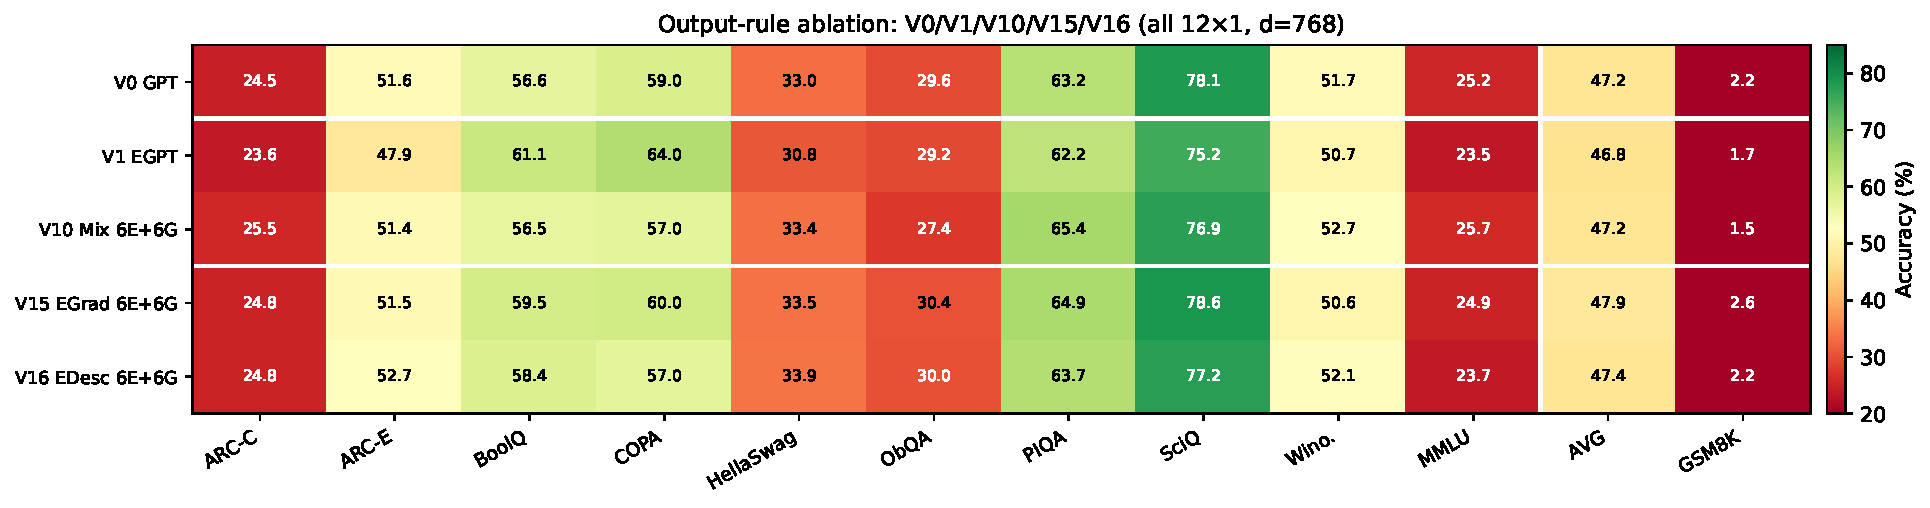
\includegraphics[width=\textwidth]{../results/multi-block-ablation/plots/new_variants_heatmap.pdf}
  \caption{Absolute accuracy heatmap for the output-rule ablation.  V15 (EGrad) and
    V16 (EDesc) are both iso-param and iso-FLOP to V10 Mixed (144M / 285 MFLOPs/tok).}
  \label{fig:new_variants_heatmap}
\end{figure}

\begin{figure}[h]
  \centering
  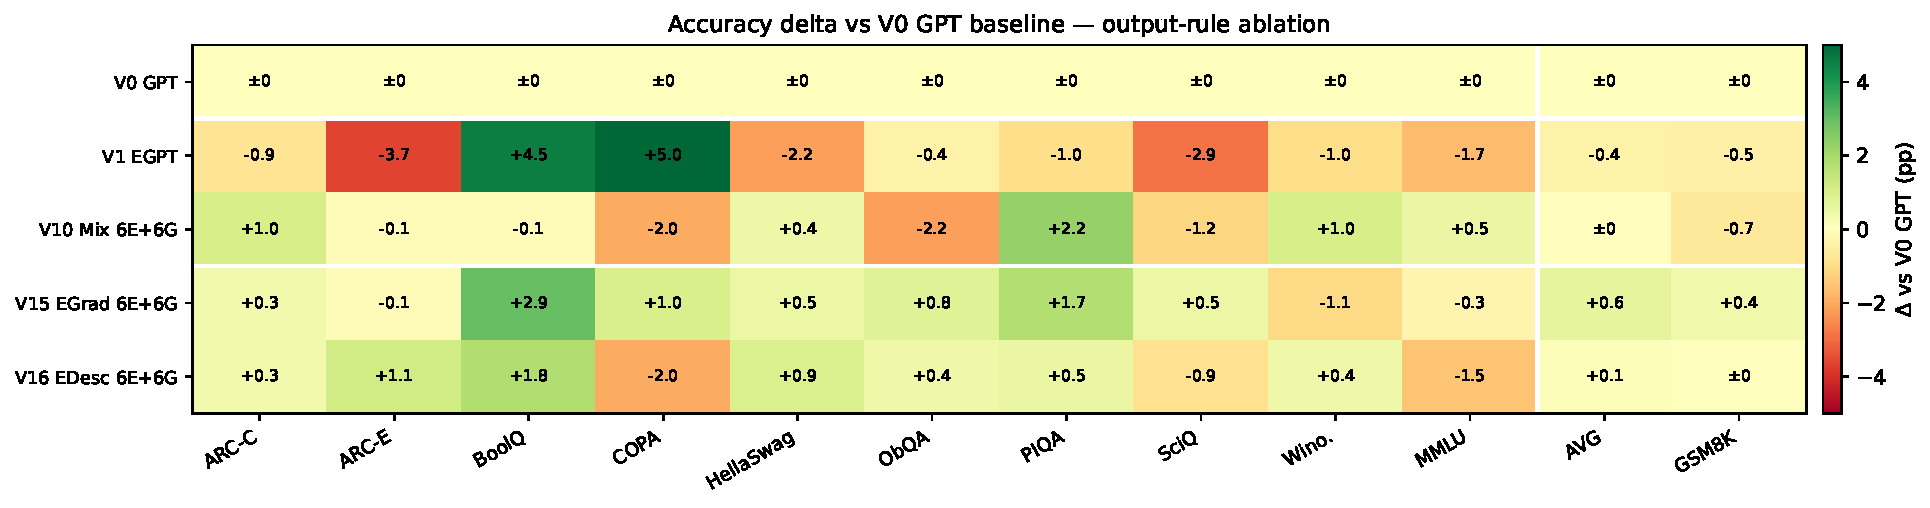
\includegraphics[width=\textwidth]{../results/multi-block-ablation/plots/new_variants_delta_heatmap.pdf}
  \caption{Accuracy delta vs.\ V0 GPT baseline.  V15 EGrad shows broad improvements
    across tasks; V16 EDesc recovers GSM8K parity with V0.}
  \label{fig:new_variants_delta}
\end{figure}

\begin{figure}[h]
  \centering
  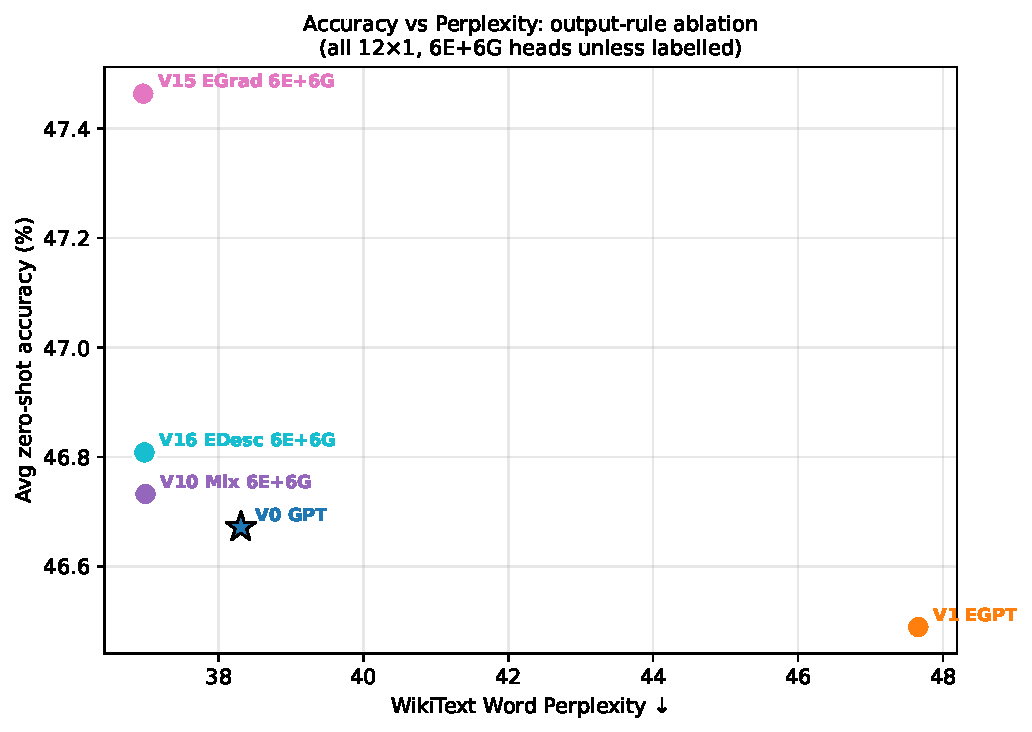
\includegraphics[width=0.6\textwidth]{../results/multi-block-ablation/plots/new_variants_ppl_vs_acc.pdf}
  \caption{Perplexity vs.\ accuracy: V15 EGrad achieves the best PPL and best avg accuracy
    simultaneously, strictly dominating V0 GPT and V10 Mixed on both axes.}
  \label{fig:new_variants_ppl_vs_acc}
\end{figure}

\paragraph{Key findings.}
\begin{enumerate}
  \item \textbf{V15 EGrad strictly dominates V10 Mixed and V0 GPT.}
    Replacing the mixed-head output with the true energy gradient
    ($W_Q^\top \mathrm{softmax}(\cdot) K$) yields 47.9\% avg accuracy
    ($+0.7$pp over V10, $+0.7$pp over V0), best PPL (36.96), and best GSM8K
    (2.58\% vs.\ V0's 2.20\%), all at 144M params / 285 MFLOPs/token.
    This is the first variant in this ablation to simultaneously beat V0 GPT on
    accuracy \emph{and} GSM8K while using fewer FLOPs.

  \item \textbf{V16 EDesc matches V0 on GSM8K and achieves competitive accuracy.}
    The energy descent rule ($h \leftarrow h - \mathrm{attn\_out}$) achieves
    47.4\% avg accuracy ($+0.2$pp over V10) and 2.20\% GSM8K (ties V0),
    with best-in-class PPL of 36.98.  The subtractive update is a modest but
    consistent improvement over additive V10 across most tasks.

  \item \textbf{Both variants recover the GSM8K regression.}
    V10 Mixed suffered a GSM8K drop relative to V0 (1.52\% vs.\ 2.20\%).
    Both V15 (2.58\%) and V16 (2.20\%) fully recover this, suggesting the
    regression was caused by the $V{=}K$ output rule of energy heads rather
    than by the mixed-head architecture itself.
\end{enumerate}

\end{document}
